\documentclass[12pt,openright,twoside]{book}
\usepackage{graphicx}
\usepackage{subcaption}
\usepackage{geometry}
\usepackage{pdflscape}
\usepackage{natbib}
\usepackage{amsmath}
\DeclareMathOperator{\sgn}{sgn}
\usepackage{amssymb}
\usepackage{pdflscape}
%%\usepackage{tabu}
\usepackage{caption}
%%\usepackage{floatrow}
\usepackage{enumerate}
\usepackage{enumitem}
\usepackage{titlesec}
\usepackage{wrapfig}
\usepackage[toc,page]{appendix}
\usepackage{lmodern}  % for bold teletype font
\usepackage{amsmath}  % for \hookrightarrow
%\usepackage{xcolor}   % for \textcolor
\usepackage[usenames,dvipsnames]{color}
\usepackage{listings}
\lstset{
    columns=fullflexible,
    frame=single,
    breaklines=true,
    postbreak=\mbox{\textcolor{red}{$\hookrightarrow$}\space},
    basicstyle=\ttfamily, 
    numbers=left, 
    numberstyle=\small\ttfamily\color{Gray},
    stepnumber=1,              
    numbersep=10pt, 
    numberfirstline=true, 
    numberblanklines=true, 
    tabsize=4,
    lineskip=-1.5pt,
    extendedchars=true,
    keywordstyle=\color{Blue}\bfseries,
    identifierstyle=, % using emph or index keywords
    commentstyle=\sffamily\color{OliveGreen},
    stringstyle=\color{Maroon},
    showstringspaces=false,
    showtabs=false,
    upquote=false,
    %texcl=true % interpet comments as LaTeX
}

\lstdefinelanguage{julia}
{
  keywordsprefix=\@,
  morekeywords={
    exit,whos,edit,load,is,isa,isequal,typeof,tuple,ntuple,uid,hash,finalizer,convert,promote,
    subtype,typemin,typemax,realmin,realmax,sizeof,eps,promote_type,method_exists,applicable,
    invoke,dlopen,dlsym,system,error,throw,assert,new,Inf,Nan,pi,im,begin,while,for,in,return,
    break,continue,macro,quote,let,if,elseif,else,try,catch,end,bitstype,ccall,do,using,module,
    import,export,importall,baremodule,immutable,local,global,const,Bool,Int,Int8,Int16,Int32,
    Int64,Uint,Uint8,Uint16,Uint32,Uint64,Float32,Float64,Complex64,Complex128,Any,Nothing,None,
    function,type,typealias,abstract
  },
  sensitive=true,
  morecomment=[l]{\#},
  morestring=[b]',
  morestring=[b]" 
}
\usepackage[utf8]{inputenc}
\usepackage{csquotes}
\usepackage{hyperref}
\hypersetup{
    colorlinks=false
}


\titleformat{\chapter}
  {\Large\bfseries} % format
  {}                % label
  {0pt}             % sep
  {\LARGE}           % before-code

\renewcommand{\figurename}{\textbf{Figure}}
\renewcommand{\tablename}{\textbf{Table}}
\newcommand{\HRule}{\rule{\linewidth}{0.4mm}}

\renewcommand{\contentsname}{{\Huge Table of Contents}}
\renewcommand{\chaptername}{{\Huge  }}
%\renewcommand{\thebibliography}{\Bibliografie}


\geometry{
 a4paper,
 total={210mm,297mm},
 left=25.0mm,
 right=25.0mm,
 top=25.0mm,
 bottom=30.0mm,
 }

 \setcounter{tocdepth}{3}
%level -1: part, 0: chapter, 1: section, etc.

\begin{document}

\begin{titlepage}
\begin{center}






\includegraphics[width=16cm]{./header.png}



\vspace{4cm}



    \HRule \\[0.3cm]


    {\Large \textsc {Simulation of Potts Model on a Dynamically Rewired Network}}\\


  \HRule \\[1.1cm]

  \textsc{\large Bachelor's Thesis}\\[4cm]

   \begin{flushleft} \large
    {Author} \\[0.1cm]
    Luca Mircea MIHĂILESCU
   \end{flushleft}

   \begin{flushright} \large
    {Scientific coordinator} \\[0.1cm]
    Conf. Univ. Dr. Alexandru NICOLIN
   \end{flushright}


  \vfill

  % Partea de jos a paginii
 %% {\large \today}

 {\large Bucharest, 2020}

\end{center}

\end{titlepage}
\newpage
\vspace*{\fill}
\thispagestyle{empty}




\newpage
\thispagestyle{plain} \pagenumbering{roman}


\vspace*{36pt}

\begin{center}

{\LARGE \textbf{Acknowledgements}}

\end{center}

\vspace{36pt}
I would like to acknowledge and thank the following important people who have supported me, not only during the course of this project, but throughout my Bachelor's degree.\\

Firstly, I would like to express my gratitude to my supervisor, Assistant Professor Dr. Alexandru Nicolin, for his support, guidance in the field of numerical methods and simulations, and insight throughout this research project.\\

I would also like to thank my colleague, Sebastian
Micluță-Câmpeanu. Without his expertise in the Julia programming language, I would not been able to run my simulations at the scale I did.\\

And finally, I would like to thank all my close friends and family. You have all helped me to focus on what has been a hugely rewarding and enriching process.\\

\vspace{40pt}

\vspace*{\fill}
\newpage
\thispagestyle{empty} \vspace*{\fill} \tableofcontents

\setlength\parindent{0pt}



\setcounter{page}{0}

%% this comand remove indent

\newpage

 \pagenumbering{arabic}


\chapter{Introduction}
\label{intro}

The understanding of the laws which govern the behaviour of social masses is one of the outstanding challenges of modern research. It is now more important than ever as our democratic societies are threatened by the rise of \textit{en masse} data mining and nontransparent social media algorithms\cite{o'neil_2016}. Fortunately, physics can lend a hand in building such an understanding. The idea of a physical modeling of social phenomena is not at all a new one. In an 1825 essay, french philosopher Auguste Comte defines social physics as:\\

\begin{displayquote}
"that science which occupies itself with social phenomena, considered in the same light as astronomical, physical, chemical, and physiological phenomena, that is to say as being subject to natural and invariable Laws the discovery of which is the special object of its researches." \cite{iggers_1959,comte_1825} 
\end{displayquote}

\vspace{14pt}

Ten years later, Belgian statistician Adolphe Quetelet publishes his \textit{Essay on Social Physics}\cite{quetelet_1835}, which proposes characterising social statistics using the concept of the 'average man' which would be built on measured variables that follow a normal distribution\cite{jahoda_2015}. After this essay, Comte would go on to refer to his new field as sociology, out of fear of being regarded as a follower.\\

The developments in the fields of social statistics were well known to Maxwell and Boltzmann and played a role in their embracing a statistical description of gases in favour of  deriving the macroscopic laws of gases from the individual motions of particles, thus laying the foundations of modern statistical physics\cite{porter}.  In a 1873 lecture to the British Association, Maxwell argues that physicists have started to employ the methods already used at the time by social statisticians\cite{maxwell_1873}. Boltzmann, in the introduction to a scientific paper published by the Vienna Academy of Science a few years earlier, similarly states that the connection between the theory of heat and 'the principle of living forces' has been "known for a long time already"\cite{boltzmann_1866}.\\

In the recent years, with the extended accessibility to computational resources and large databases (mostly thanks to the Internet), the field of social dynamics has made the transition from philosophical thought experiments to concrete research efforts worldwide\cite{castellano_fortunato_loreto_2009}. However, to apply the tools and concepts of thermodynamics to the study of society, one needs to understand their meaning in a social context. One such interpretation of thermodynamics concepts into sociology has been produced by J. Mimkes in 1995 \cite{mimkes_1995}. According to his study, a binary multicultural society can be understood using the model of regular solutions, which is applied to metal alloys. Members of two communities can manifest sympathy to members outside the community (attractive interaction), be indifferent to them (ideal solution), or manifest antipathy to them (repulsive interaction). In this interpretation Gibbs free energy G describes the general happiness of the society, and temperature T can be understood as tolerance, which can make society more united against the differences of the two communities. Table ~\ref{mimkes} shows all the conclusions drawn regarding the equivalence between thermodynamics and social science.\\

\begin{table}[!ht]
\centering
\begin{small}
\caption{\textit{Equivalence of thermodynamics terms to social science according to Mimkes' model of regular mixtures}}
\begin{tabular}{ccc}

\hline\hline
Abbreviation  & Natural Science & Social science\u{a}      \\
\hline
A-B           & Alloys                  & Societies   \\
$x$           & atomic percentage       & size of minority (\%)  \\
              & \underline{Functions}   & \underline{Feelings} \\
$G$           & free enthalpy           & general happiness   \\
$T$           & temperature             & tolerance  \\
$E_{AA}$      & cohesive energy         & tradition, heritage\\
$E_{AB}>0$    & cohesive energy         & curiosity, love   \\
$E_{AB}<0$    & repelling energy        & distrust, hate  \\
$E=0$         & no cohesion             & apathy  \\
$\epsilon>0$  & attractive interaction  & sympathy  \\
$\epsilon=0$  & ideal solution          & indifference          \\
$\epsilon<0$  & repelling interaction   & antipathy  \\
              & \underline{State of alloys}         & \underline{State of Society}  \\
              & disorder, solubility    & integration  \\
              & solubility limit        & segregation  \\
              & phase diagram           & intermarriage diagram  \\

\hline \label{mimkes}
\end{tabular}
\end{small}
\end{table}




\section{The Ising paradigm}

Whether we're focusing on opinions, social status, cultural and linguistic features, or human kinematics, models can be devised in terms of small sets of variables. Of course, they would be oversimplifications, but qualitative properties of large scale phenomena do not necessarily depend on the microscopic details of the process. As such, simplified models can offer valuable information about macroscopic features such as symmetries, dimensionality, conservation laws etc. One of the most relevant models in physics to this kind of analysis is the Ising model for ferromagnets\cite{binney_2002}. Beyond its physical significance, the Ising ferromagnet can also serve as a simple model for opinion dynamics: spins can be seen agents under the influence of the majority of their interacting partners.\\

Let us consider a collection of $N$ points (i.e. agents) with a spin (i.e. opinion) $s_i=\pm1$. For any two neighbouring points $i,j$ there is an interaction $J_{ij}$. Energetically, this interaction determines each spin to be aligned with its nearest neighbours. When no external magnetic field is present, the total energy of the system is equal to the Hamiltonian function

\begin{equation}
H=-\frac{1}{2}\sum_{(i,j)}J_{ij}s_is_j
\label{ising-hamiltonian}
\end{equation}

\vspace{14pt}

where the sum runs on the pairs of neighbours. The most common implementation of the Ising dynamics is the Metropolis algorithm\cite{landau_binder_2015}. In it, each step of the simulation a spin is flipped with a probability exp($-\Delta E/k_BT$), where $\Delta E$ is the change in energy, $k_B$ is the Boltzmann constant, and $T$ is the temperature. The interactions driven by (\ref{ising-hamiltonian}) should lead to a completely homogeneous state: either all spins are positive, or all are negative. However, this holds only for small temperatures. At temperatures above a critical temperature $T_c$, thermal noise injected fluctuations destroy order. By definition, the average magnetization is\\

\begin{equation}
M=\frac{1}{N}\sum_j\langle s_j \rangle
\label{ising-magnetization}
\end{equation}

\vspace{14pt}

where the brackets denote the average over different iterations. For $T<T_c$ the magnetization will be $M(T)>0$, while for $T>T_c$, $M(T)=0$. Worth mentioning is also the Potts model\cite{wu_1982}, which will be relevant later on for the model I decided to employ. The difference in its case is that spins can take one out of $q$ values. Identical neighbouring spins are energetically favored. The Potts has found such uses as the simulation of sorting in a mixture of biological cells\cite{graner_glazier_1992}, or computer vision and image restoration\cite{boykov_veksler_zabih_2001}. The Ising model corresponds to the Potts special case $q=2$.\\

\begin{figure}
\centering
\begin{subfigure}[b]{0.3\linewidth}
    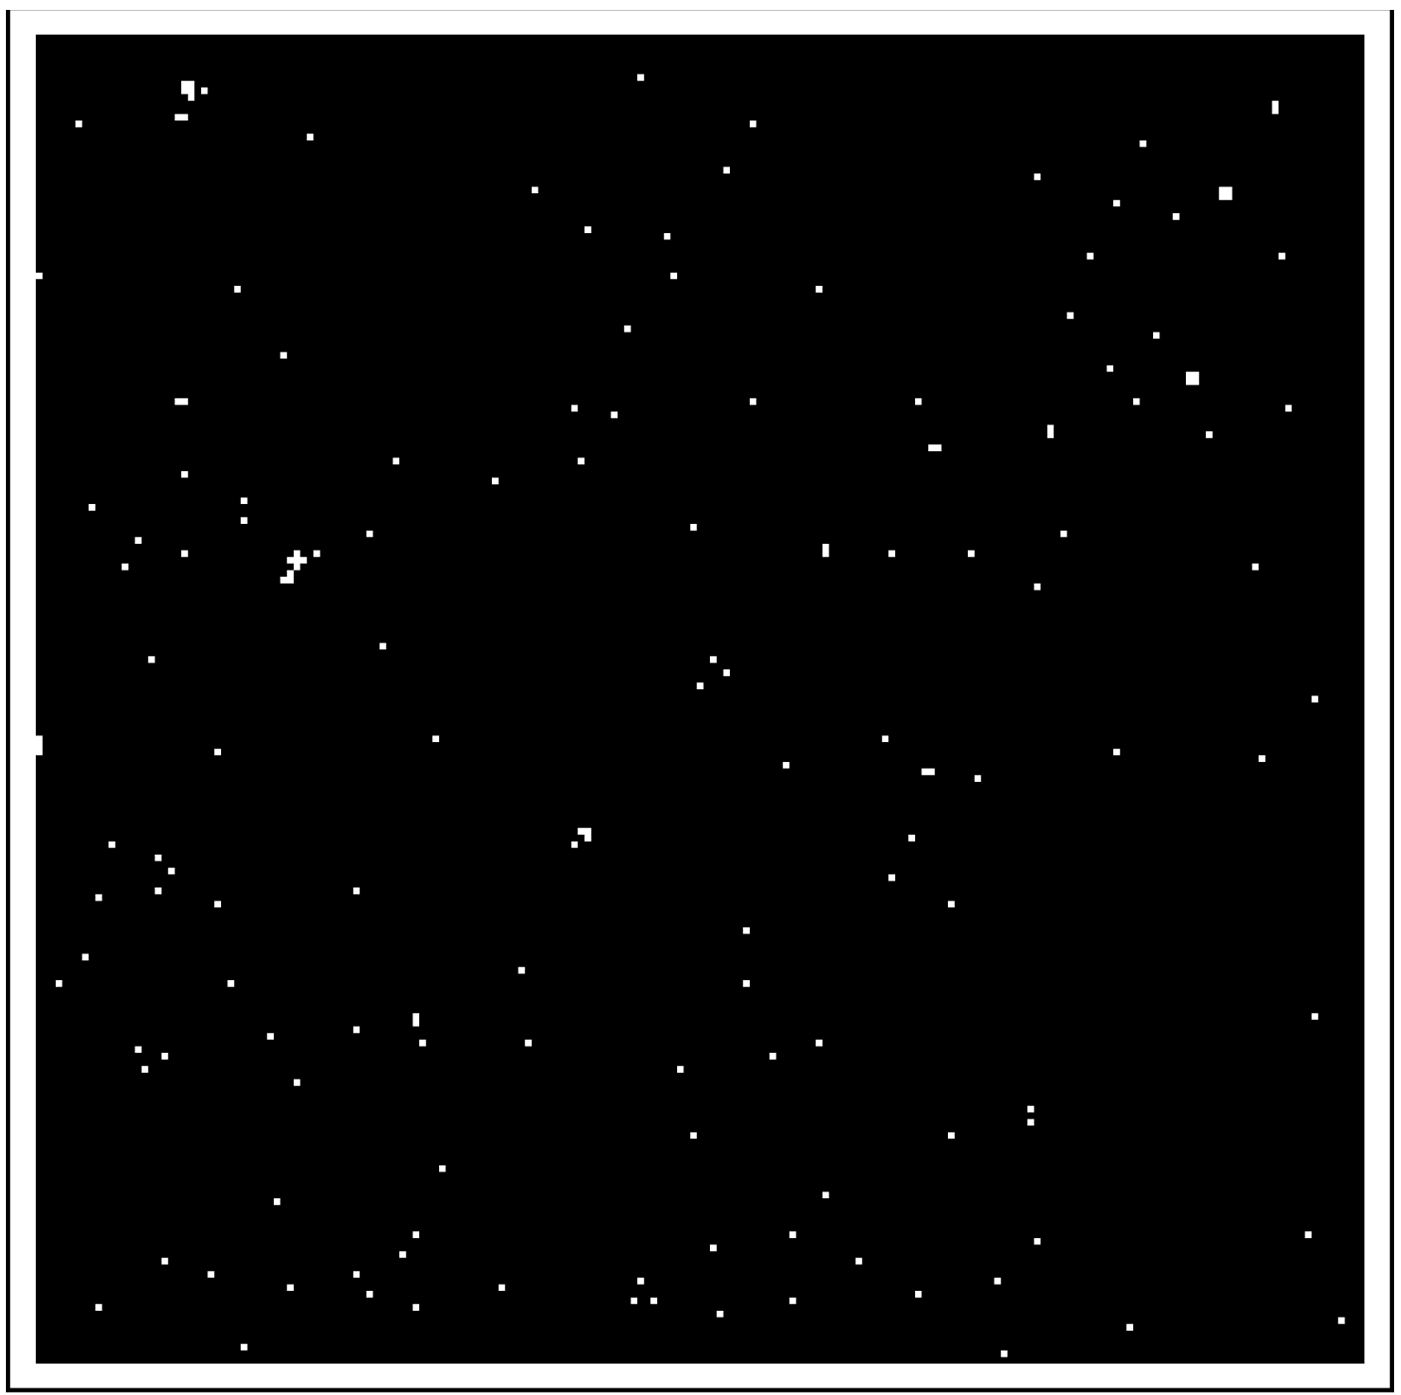
\includegraphics[width=\linewidth]{figures/t<t_c.PNG}
    \caption{$T<T_c$}
\end{subfigure}
\begin{subfigure}[b]{0.3\linewidth}
    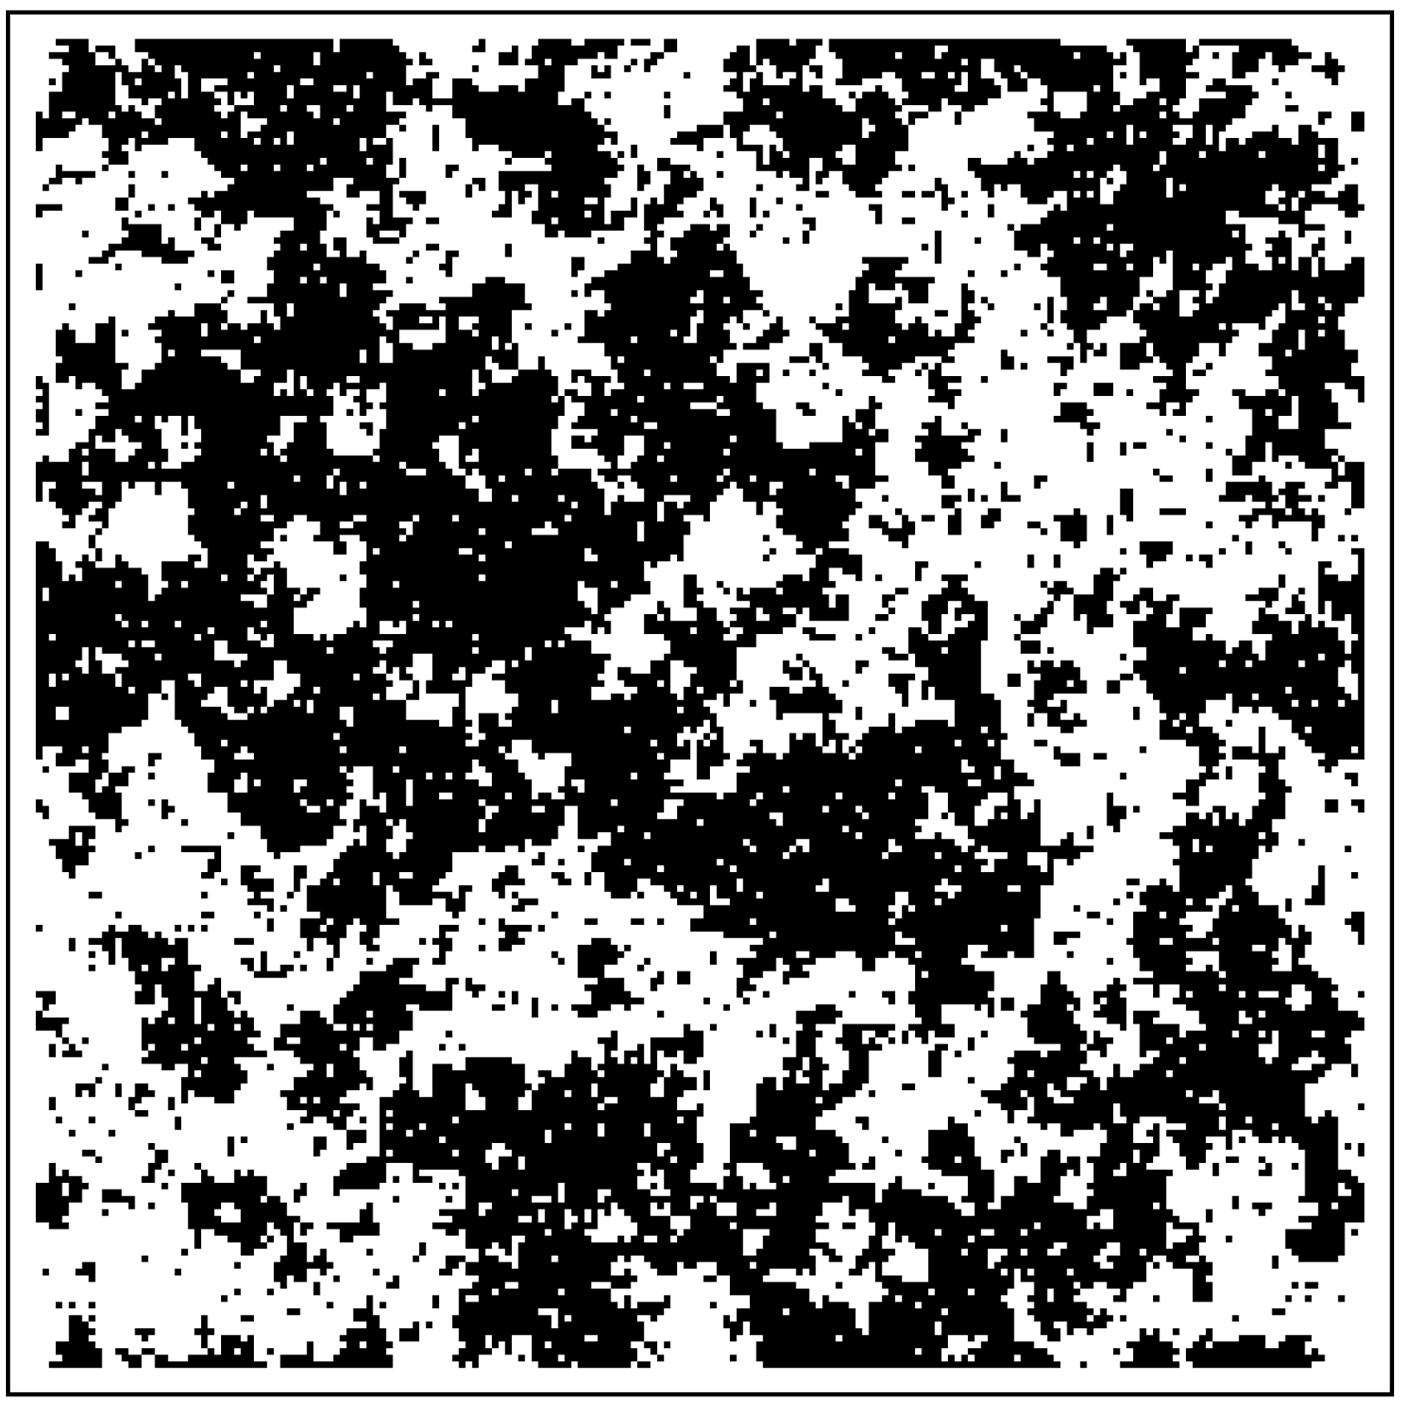
\includegraphics[width=\linewidth]{figures/t=t_c.PNG}
    \caption{$T\sim T_c$}
\end{subfigure}
\begin{subfigure}[b]{0.3\linewidth}
    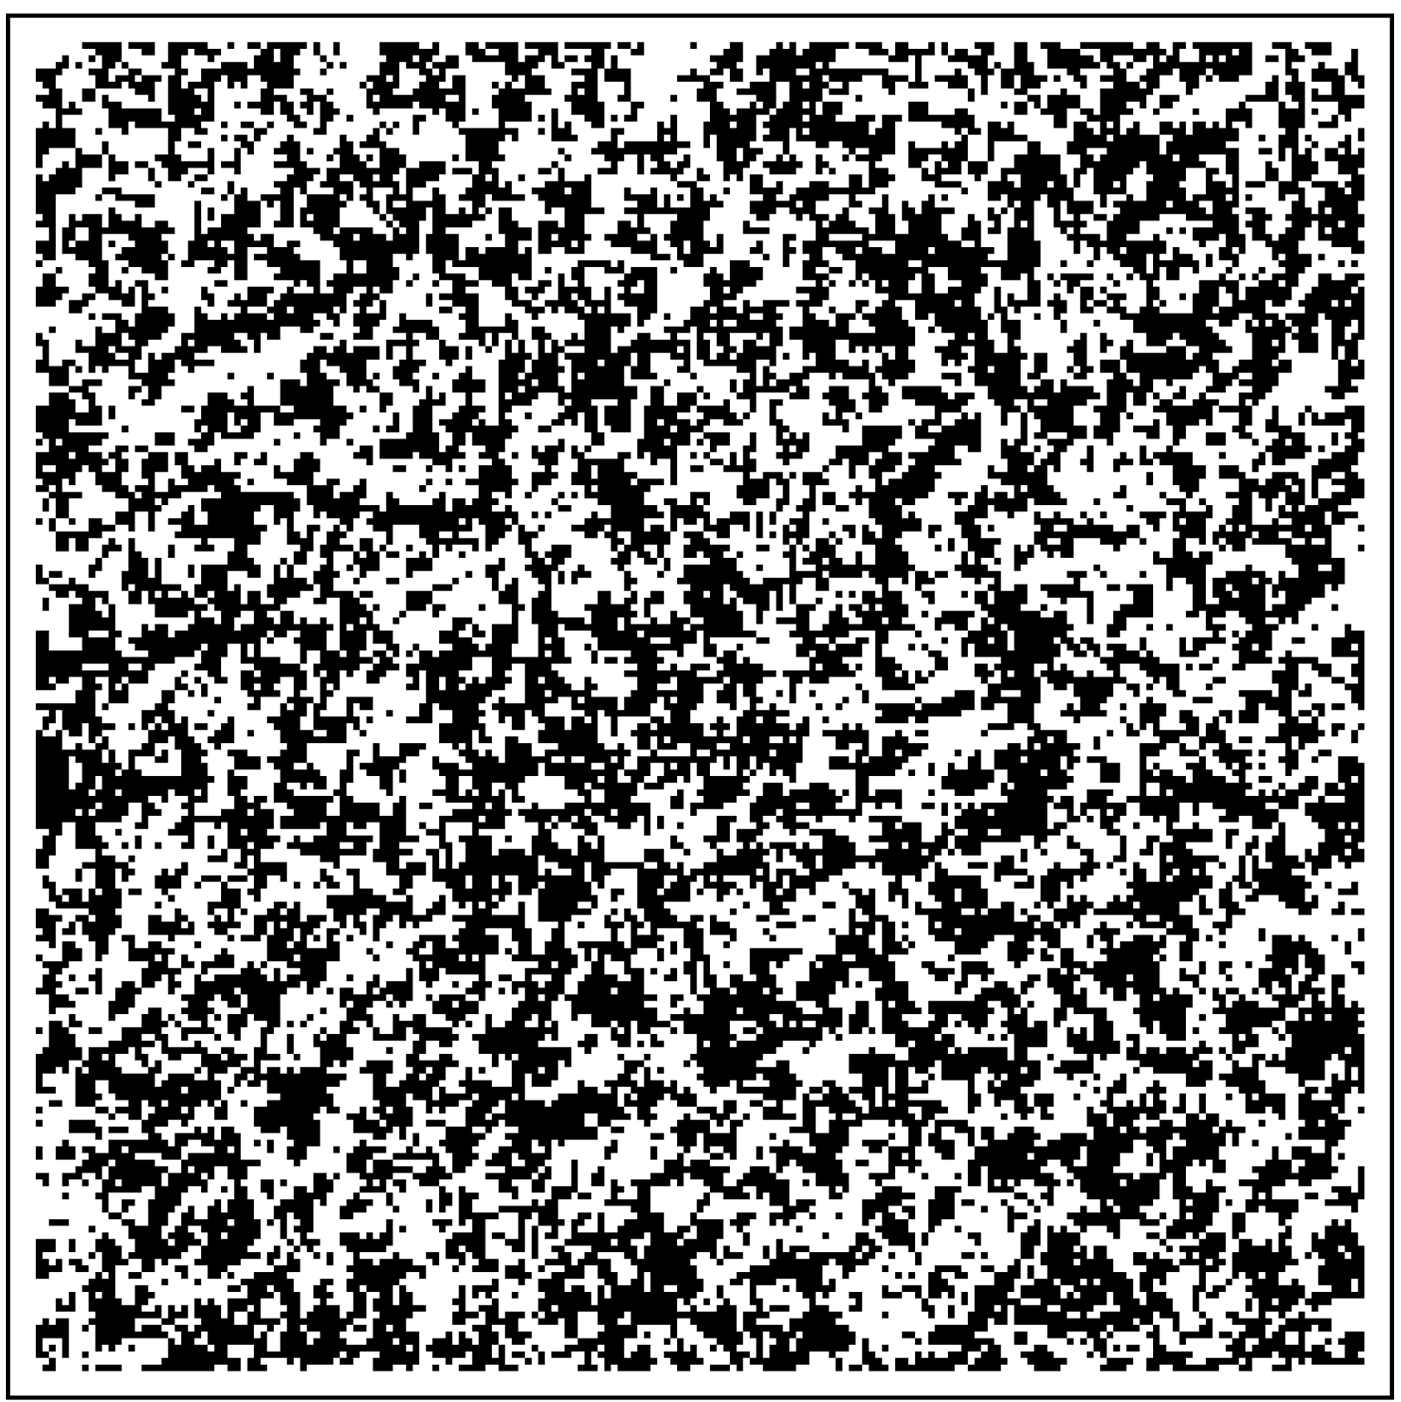
\includegraphics[width=\linewidth]{figures/t>t_c.PNG}
    \caption{$T>T_c$}
\end{subfigure}
\caption{\textit{{\small Spatial configurations in the Ising model. Black squares represent spins with $\sigma=+1$ and white one correspond to $\sigma=-1$. (Reprinted from "Behavior of Early Warnings near the Critical Temperature in the Two-Dimensional Ising Model," by Morales I.O., Landa E., Angeles C.C., Toledo J.C., Rivera A.L., et al., 2015, PLOS ONE, 10(6), doi:10.1371/journal.pone.0130751. Copyright 2015 by Morales et al. Distributed under terms of the Creative Commons Attribution License.)}}}
\label{quench}
\end{figure}

Yet another variation to the Ising model can be found in Axelrod's model of dissemination of culture\cite{axelrod_1997}. From the point of view of statistical physics it is a vectorial generalization of the Ising-like models (here culture refers to a vector of variables denoting a set of inextricable 'cultural' characteristics). The model consists of individuals located on a network (or lattice) endowed with a vector of F integer variables $(\sigma_1,...,\sigma_F)$. Each variable, or 'cultural features', can assume values $\sigma_f=0,1,...,q$. These cultural features are supposed to model different “beliefs, attitudes, and behavior”. Each step, an individual $i$ together with a neighbor $j$ are selected and the similarity between them is calculated:\\

\begin{equation}
\omega_{i,j}=\frac{1}{F}\sum^F_{f=1}\delta_{\sigma_f(i),\sigma_f(j)}
\label{axelrod-probability}
\end{equation}

\vspace{14pt}

here $\delta_{i,j}$ being Kronecker's delta. Then, with probability $\omega_{i,j}$ one of the features for which traits are different is set equal to the neighbor's ($\sigma_f(i)=\sigma_f(j)$). The phenomenology these dynamics determine is not trivial, however, and predicts the emergence of polarization despite the tendency of interacting people to become more alike.

The Ising model has been applied to describe business confidence, segregation, and language change\cite{stauffer_2008}. In the last two cases\cite{schelling_1971,nettle_1999}, the authors were not aware of the Ising model, and designed more complex simulations that were less flexible. In the case of business confidence\cite{hohnisch_pittnauer_solomon_stauffer_2005} good news or bad news can lead to a uniform optimist or pessimist overlook in the population, if the news follow in too quick succession (i.e. the field oscillates too much), people will start ignoring them and adopting random opinions \cite{hohnisch_stauffer_pittnauer_2008}. In the study of segregation, temperature T emerges as a measure of tolerance, with individual agents possibly having their own T which might change over time. In the case of language change, it seems that the rate of change for certain characteristics decays as the population gets larger. If the agents only exchange characteristics with their neighbours, this influence is weak.\\

\section{Scale-free distributions}

A very important role in the theory of critical phase transitions (such as the one reviewed earlier in the case of the Ising model) is played by critical point exponents\cite{yeomans_1992}. To arrive to critical exponents, we need to define, for convenience, a measure of the deviation in temperature from the critical temperature $T_c$:\\

\begin{equation}
\tau=\frac{T-T_c}{T_c}
\label{deviation-critical}
\end{equation}

\vspace{14pt}

The critical exponent associated with a function will then be:\\

\begin{equation}
\lambda=\lim_{\tau\to 0}\frac{\ln|F(\tau)|}{\ln|\tau|}
\label{critical-exponent}
\end{equation}

\vspace{14pt}

More usually, we will encounter the following, equivalent, relation:\\

\begin{equation}
F(\tau)\sim |\tau|^{-\lambda}
\label{critical-exponent-relation}
\end{equation}

\vspace{14pt}

Here, the $\sim$ sign is used instead of the two sides being equal because (\ref{critical-exponent-relation}) it represents the asymptotic behaviour of the function $F(\tau)$ as $\tau \to 0$. In magnetic systems, critical exponents are for several functions, some of the most common of which are listed in table ~\ref{magnetic-functions}.\\

\begin{table}[!ht]
\centering
\begin{small}
\caption{\textit{Commonly used critical exponents for a magnetic and fluid systems}}
\begin{tabular}{ccc}

\hline \hline
Magnetic system\\
\hline
Zero-field specific heat             & $C_H\sim|\tau|^{-\alpha}$   \\
Zero-field magnetization             & $M\sim(-\tau)^{\beta}$ \\
Zero-field isothermal susceptibility & $\chi_T\sim|\tau|^{-\gamma}$\\
Critical isotherm ($t=0$)            & $H\sim|M|^{\delta}\sgn (M)$ \\
Correlation length                   & $\xi\sim|\tau|^{-\nu}$ \\
Pair correlation function at $T_C$   & $G(\Vec{r})\sim 1/r^{d-2+\eta}$ \\
\hline
Fluid system\\
\hline
Specific heat at constant volume $V_C$& $T\sim |t|^{-\alpha}$\\
Liquid-gas density difference & $(\rho_l-\rho_g)\sim(-t)^\beta$\\
Isothermal compressibility & $k_T\sim|t|^{-\gamma}$\\
Critical isotherm ($t=0$) & $P-P_c\sim|\rho_l-\rho_g|^\delta\sgn(\rho_l-\rho_g)$\\
Correlation length & $\xi\sim|\tau|^{-\nu}$\\
Pair correlation function at $T_C$   & $G(\Vec{r})\sim 1/r^{d-2+\eta}$ \\
\hline
\label{magnetic-functions}
\end{tabular}
\end{small}
\end{table}




We call a distribution scale-free when it follows a power law like the one at (\ref{critical-exponent-relation}). Essentially, when measuring something, if the distribution of results follows a power-law it means that the measured phenomenon exhibits features at all scales. This occurrence is not at all limited to critical phase transitions, however\cite{pinto_lopes_machado_2012}. For example, the distribution of earthquake magnitudes seems to obey a $k^{-\gamma}$ function with $\gamma\approx3.04$, number of hits on web sites, $\gamma\approx2.40$, intensity of wars, $\gamma\approx1.80$, and intensity of solar flares, $\gamma\approx1.83$ \cite{newman_2005}. Studies have also been done on the rank-frequency distribution of words in various languages, of which I will just mention Romanian, with $\gamma\approx1$ \cite{cocioceanu_raportaru_nicolin_jakimovski_2017}, and English, with $\gamma\approx2.20$ \cite{newman_2005}.\\

Scale-free distributions do not need to follow strictly a $k^{-\gamma}$ form. Take, for instance, figure \ref{power-law-distribs}, which comes from a study calculating the distribution of income in the United States\cite{toda_2012}. The distribution in this case is a double power law. More complex distributions exist, but they are beyond the scope of this thesis.\\

\begin{figure}[!htb]
\centering
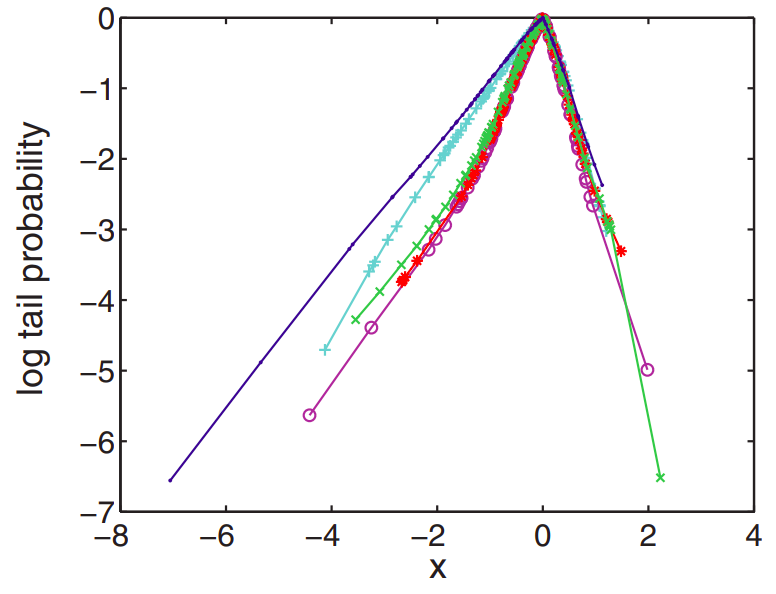
\includegraphics[width=0.65\linewidth]{figures/income_distribution.png}
\caption{\textit{{\small Laplace plot by age group. Cyan plus (+): under 30, magenta circle (o): 30s, red asterisk (*): 40s, green cross (x): 50s, blue dot (·): over 60. Data from the U.S. Census Bureau Current Population Survey 2000-2009. Reprinted from Journal of Economic Behavior \& Organization, 84(1), Alexis Akira Toda, "The double power law in income distribution: Explanations and evidence," pages 364-381, Copyright 2012, with permission from Elsevier.}}}
\label{power-law-distribs}
\end{figure}

\section{Scale-free networks}

Often, natural and man-made systems (e.g. the Internet, citation networks, social networks) have the tendency to exhibit a structure closely resembling scale-free networks\cite{barabasi_2002}. These are networks with a scale-free degree distribution (i.e. the probability that a randomly chosen node will have  $k$ connections). This means that the fraction $P(k)$ of nodes of degree $k$ has the following form:\\

\begin{equation}
P(k) \sim k^{-\gamma}
\label{scale-free}
\end{equation}

\vspace{14pt}

In a famous study about the World Wide Web, University of Notre-Dame researchers mapped all incoming and outgoing links in the university's \textit{nd.edu} domain\cite{barabasi_albert_jeong_2000}. Sure enough, the distribution they found was a power-law like the one at (\ref{scale-free}), meaning it was a scale-free network. The resulting exponent for outgoing links was then checked against the ones obtained by independently mapping \textit{whitehouse.gov}, \textit{yahoo.com}, and \textit{snu.ac.kr}. All the three domains exhibited a distribution with the same exponent as with \textit{nd.edu}, $\gamma\approx2.45$.\\

\begin{figure}[!htb]
\centering
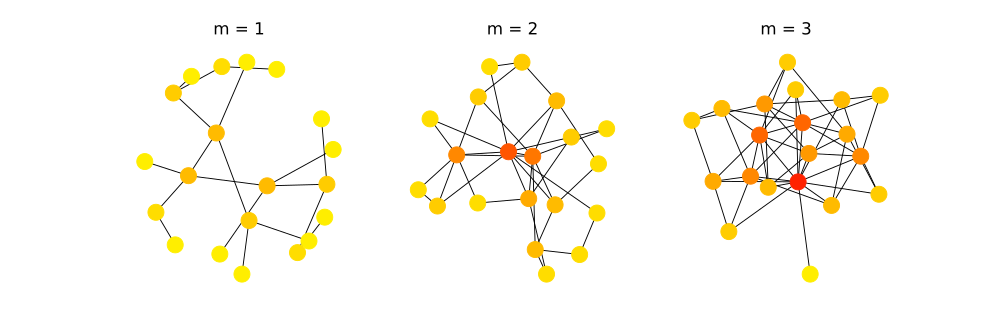
\includegraphics[width=\linewidth]{figures/1000px-Barabasi_albert_graph.png}
\caption{\textit{{\small Display of three graphs generated with the Barabasi-Albert (BA) model. Each has 20 nodes and a parameter of attachment $m$ as specified. The color of each node is dependant upon its degree (same scale for each graph). (Wikipedia user HeMath / Creative Commons Attribution-Share Alike 4.0 International license (\url{https://commons.wikimedia.org/wiki/File:Barabasi_albert_graph.svg}))}}}
\label{barabasi-graph}
\end{figure}

In an attempt to explain the occurrence of scale-free networks in real life, Albert-László Barabási and Réka Albert have elaborated an algorithm for generating random scale-free networks (see figure ~\ref{barabasi-graph}) using a preferential attachment mechanism\cite{barabasi_albert_1999}. In the Barabási-Albert model, the network starts with $m_0$ initial connected nodes. Then, new nodes are added to the network one by one. Each new node is then attached to $m \le m_0$ of the already existing nodes with the following probability:\\

\begin{equation}
p_i=\frac{k_i}{\sum_jk_j}
\label{attachment-probability}
\end{equation}

\vspace{14pt}

where $p_i$ is the probability that the new node is attached to node $i$, $k_i$ is the degree of node $i$, and the sum is calculated over all pre-existing nodes $j$.\\

An evolving Barabási-Albert network can be mapped to a Bose gas, with nodes corresponding to energy levels, and links to particles\cite{bianconi_barabasi_2001}. For each new node, $2m$ particles are added: $m$ particles on the energy level corresponding to the node's fitness, and m particles distributed to the other energy levels, corresponding to the outgoing links. There are 3 possible behaviours:\\
\begin{enumerate}
  \item Scale-free phase: occurs when all nodes have the fitness. The fraction of links of the oldest node decay to zero in the thermodynamic limit. 
  \item Fit-get-rich: occurs when nodes have different fitnesses and $I(\beta,\mu)=1$ has a solution. Eventually, the system evolves to a configuration of a few very connected nodes along with many less connected ones. 
  \item Bose-Einstein condensation: occurs under a critical temperature where $I(\beta,\mu)=1$ has no solution. Under this circumstance a winner-takes-all scenario occurs (the biggest hub also maintains a finite share of the links throughout the expansion of the system).
\end{enumerate}

\vspace{14pt}

\section{Social networks}

At the most basic level, a social network is a structure made up of a set of social actors (be it individuals or organizations), links between pairs of people (dyadic ties), and other social interactions\cite{hancean_2014,carrington_scott_2014}. Besides dyads, which are links between two people and simplest possible feature in a social network, we can also encounter repeating structures made up of three or more people. All these are called network motifs: recurrent and statistically significant patterns in a network.\\

\begin{figure}
\centering
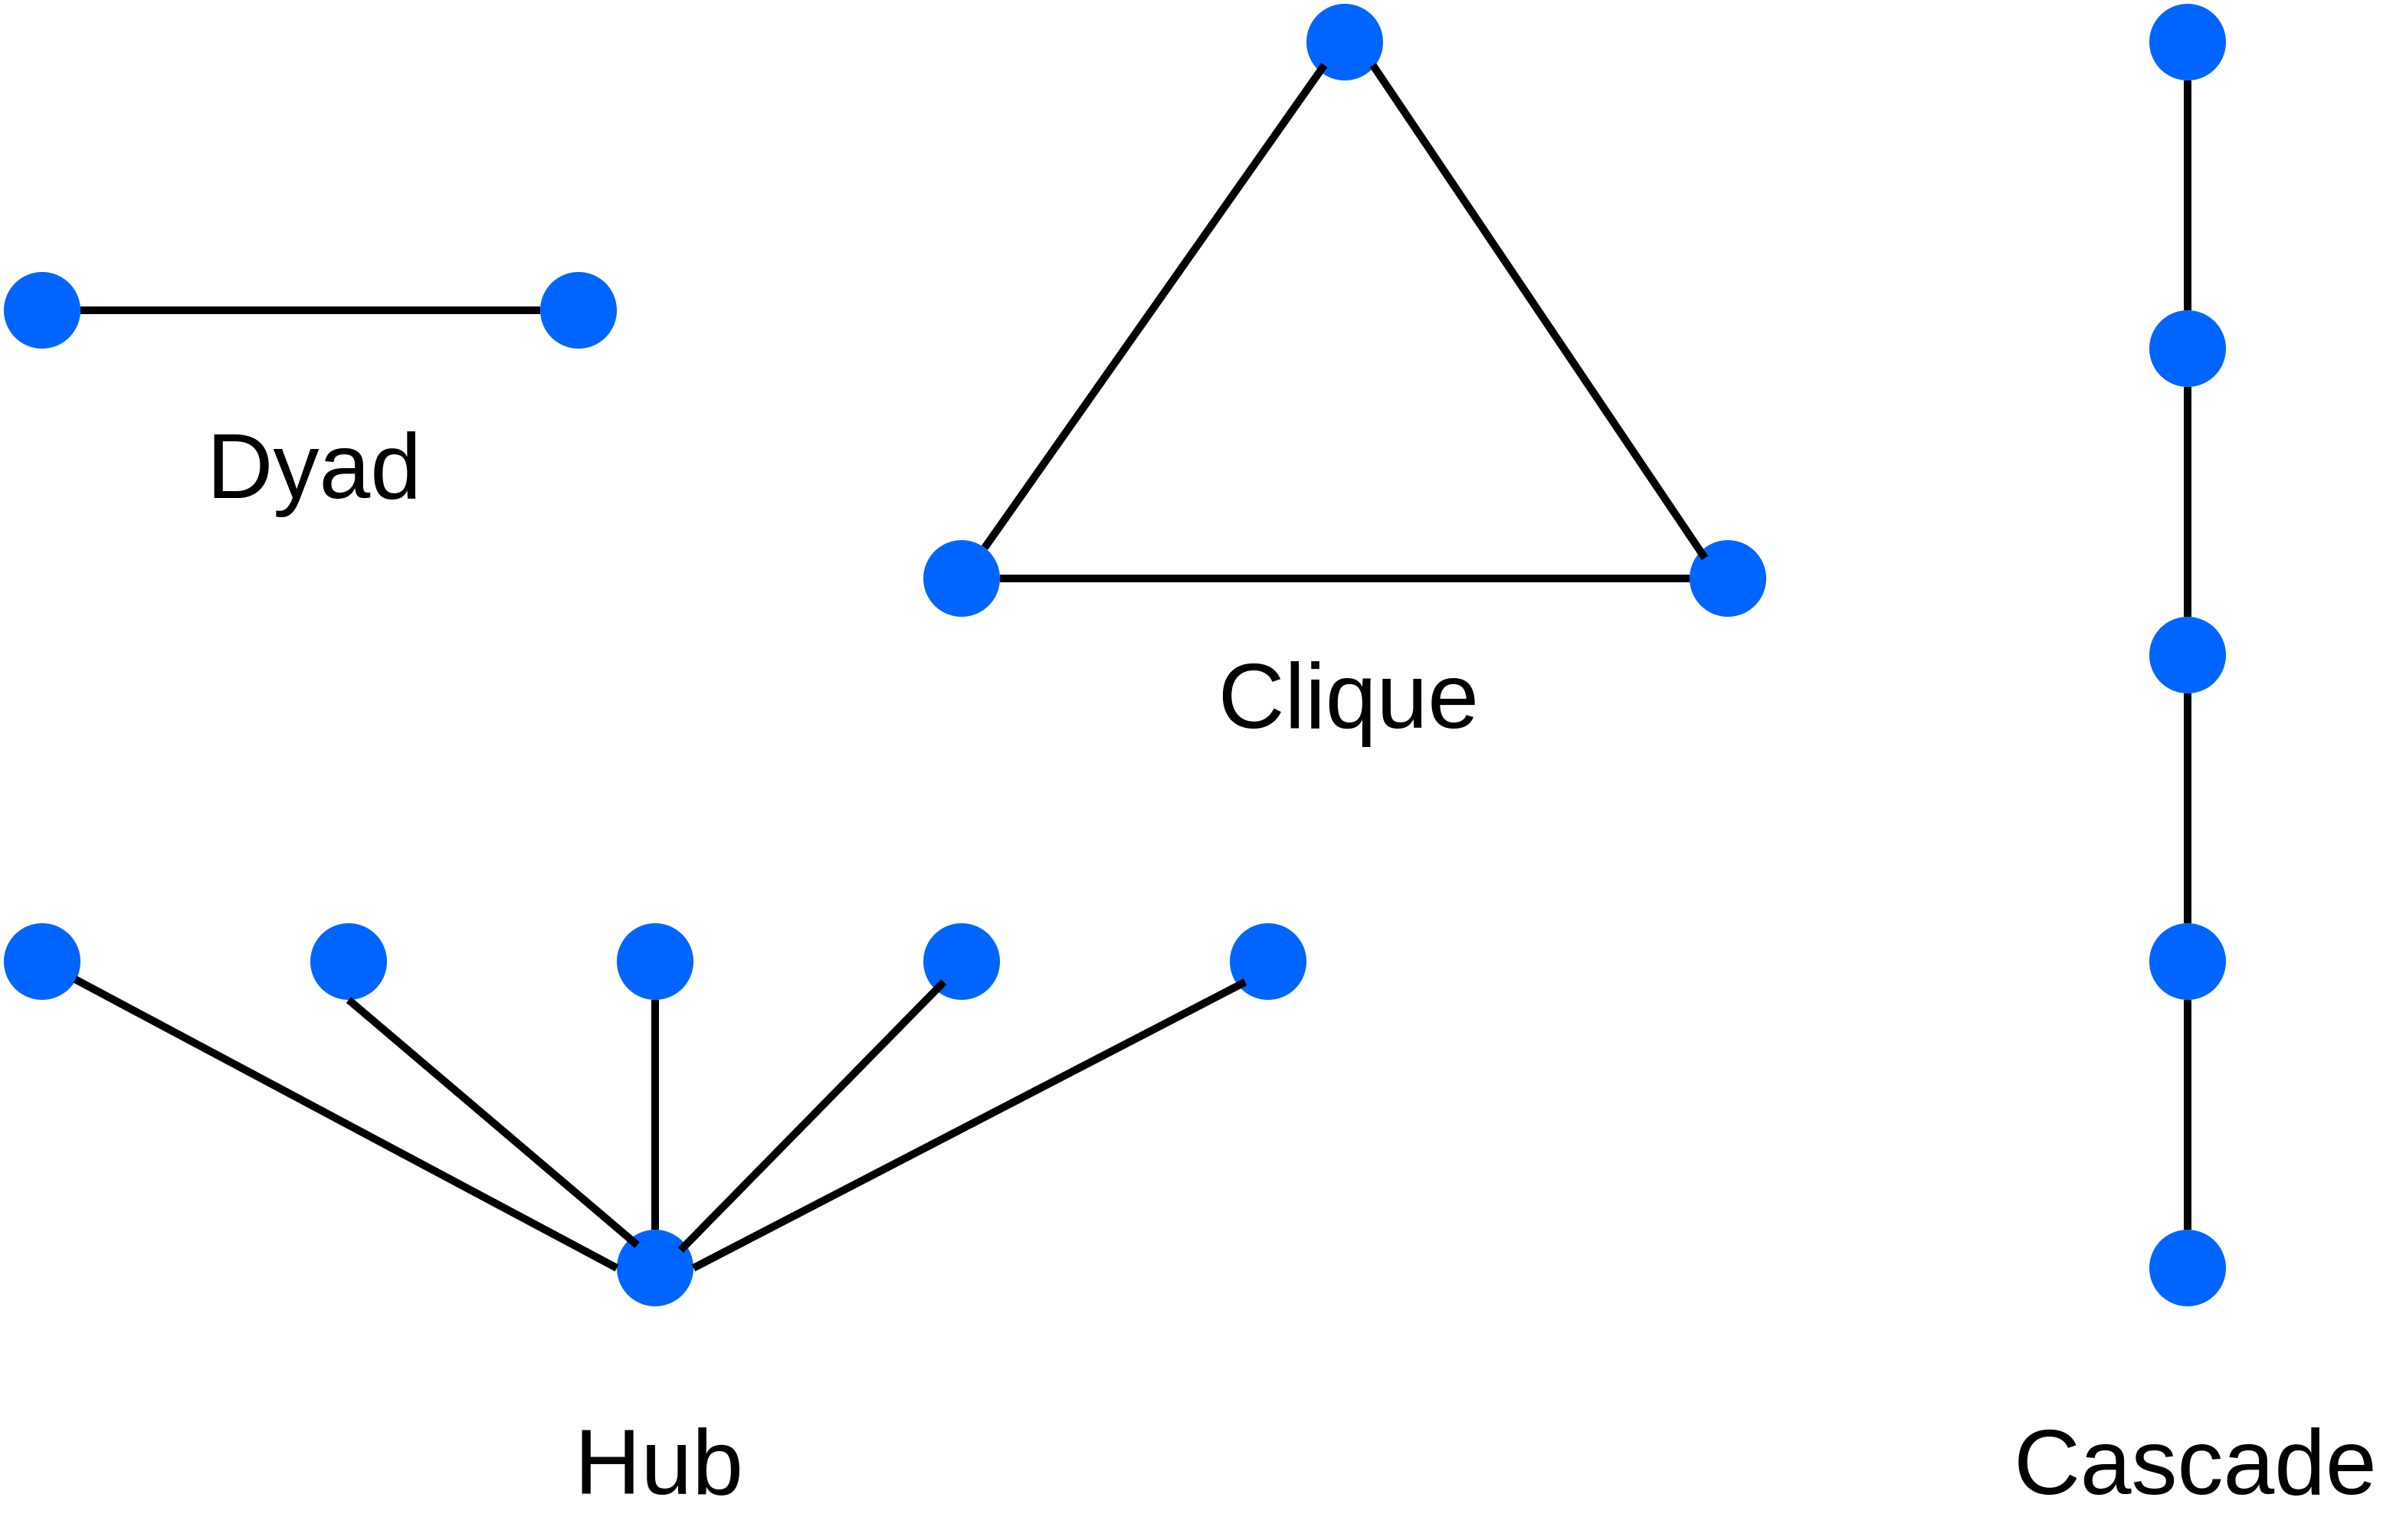
\includegraphics[width=7cm]{figures/network_motifs.png}
\caption{\textit{{\small Types of network motifs.}}}
\label{fig1}
\end{figure}

Heider's Balance Theory\cite{heider_1958} is one of the most famous theories concerned with the analysis of triads (i.e. structures emerging between tree agents).  According to it, balance state over a dyad occurs if the two like each other or dislike each other. Meanwhile, should the two have different sentiments regarding each other (positive and negative) the dyad is in imbalance. In the case of triads, balance state between the three can be found if the algebraic multiplication of signs in the triad relations has a positive sign. As it is immediately apparent, this theory holds many similarities with the aforementioned Ising dynamics, in which the energetic tendency is towards what Heider would call balance.\\

Another aspect that has been studied in social networks is the degree of separation, or average path length\cite{newman_barabasi_2006}. Arguably the most famous experiment in this area is Milgram's small-world experiment\cite{milgram_1967}. Long before the appearance of internet social networks, this experiment aimed to find what is the average path length between any two persons by making use of the postal system. The procedure was as follows:\\

\begin{enumerate}
    \item Individuals in the U.S. city of Boston, Massachusetts, were chosen to be end points of the experiment.
    \item Information packets containing the instructions for participating in the experiment were initially sent to randomly selected individuals in Omaha or Wichita.
    \item Recipients were asked to sign the roster included in the packet and resend the packet to the target person if they knew the target on a first name basis. If not, they were asked to send it to the person they deemed most likely to be able to reach them in this manner.
    \item Upon arrival, the target would inspect the roster and count how many times the package had been forwarded.
\end{enumerate}

\vspace{14pt}

Using this methodology, Milgram was able to calculate that the median number of intermediate persons was only $5.5$ \cite{barabasi_six_degrees_2002}.\\

\section{Justification for a two-layered model}

All the social simulation models reviewed thus far concerned themselves with reviewing the evolution of one observable in the system, be it opinion, cultural vector, or connectivity. Some of them equip the agents with a certain 'fitness' value, which determines the probability the agent will have influence on another agent or not. But this too is arbitrary. In real life scenarios such as elections\cite{luca_ispas_teaca_iavita_andreescu}, there is one one rapidly evolving question of opinion (e.g. candidate to vote for) while the structure of the social network is given by other, more long-term, features of the individuals (e.g. political values). In other words, one will be more likely to copy the opinion of people sharing the same values as oneself. This effect has been especially observed in the case of social media, where the followed-follower dynamic makes it easier to select the people sharing similar values\cite{holone_2016}.\\

In terms of a simulation, this considerations will translate into a two-layered model, with two different dynamics: one layer is concerned with rewiring the network so that agents with similar values connect with each other, and another layer for the evolution of the opinion of interest on said network.\\

\chapter{Model Setup}

In this thesis, I model opinion dynamics by using a Potts-like agent-based model, and the evolution of the network structure is performed by using a slightly modified version of Axelrod's model of dissemination of culture. This chapter provides the reader with a detailed description of the proposed model.\\

\section{Agent characteristics}

A directional network consisting of N agents is used. Each agent is represented by a vertex in the network, accompanied by a set of three features. These features are:\\

\begin{enumerate}
  \item \textbf{Vote:} a variable in the range of $v=0..n$, representing the agent's opinion. \textit{Votes} can be understood literally, as voting intention in an election, or, more generally, as an opinion subject to quick change in a social network.
  \item \textbf{Cultural vector:} a vector $\sigma=(\sigma_1,...,\sigma_F)$, with $\sigma_f=0,1,...,q$, representing an immutable set of cultural characteristics. Here culture is understood as, in Axelrod's words, "\textit{the set of individual attributes that are subject to social influence}".
  \item \textbf{Energy:} defined as $\epsilon_{i}=-J\sum_{j}\delta{v_i,v_j}$, where $j\in$ inneighbors, and $\delta$ is the Kronecker delta symbol. Note that this definition is akin to the Potts model Hamiltonian, with the difference that in this case spins are replaced by \textit{votes}.
\end{enumerate}

\vspace{14pt}

\section{Network rewiring}

Each step, an agent is selected for which, with a certain probability, an inneighbour will be removed and another added. Here, I referred to the transition probability defined by Axelrod for his model of dissemination of culture:\\

\begin{equation}
\omega_{i,j}=\frac{1}{F}\sum_{f=1}^{F}\delta_{\sigma_f(i),\sigma_f(j)}
\label{ax_trans_prob}
\end{equation}

\vspace{14pt}

However, this probability only grows when to cultural characteristics are \textit{identical}. In reality, beliefs are usually on a spectrum of intensity. For instance, a person with a belief $\sigma_f=3$ will find themselves more likely to interact with another with $\sigma_f=4$ rather than one with $\sigma_f=9$. Taking this into consideration, a new function $\eta$ can be devised:\\

\begin{equation}
\eta_{i,j}=1-\frac{1}{F} \cdot \frac{1}{q}\sum_{f=1}^{F}|\sigma_f(i)-\sigma_f(j)|
\label{trans_prob}
\end{equation}

\vspace{14pt}

Using this revised probability, this stage in the time-step is defined by the following activities:\\

\begin{itemize}
    \item One agent $i$ is selected at random.
    \item Another agent $j$ that is not an inneighbour is selected randomly.
    \item With a probability $\eta_{i,j}$ an edge from $j$ to $i$ is added, and $i$'s energy $\epsilon_i$ is reevaluated.
    \item Now an agent $k$ is selected randomly from $i$'s inneigbours.
    \item With a probability $1-\eta_{i,j}$ the edge from $k$ to $i$ is removed, and $i$'s energy $\epsilon_i$ is reevaluated. 
\end{itemize}

\vspace{14pt}

It is immediately apparent that this rewiring procedure will lead to similar agents becoming more connected, and eventually forming hubs. This behaviour mirrors the echo-chamber effect observed in social media.\\

\section{Opinion dynamics}

Having rewired the network the selected agent's connections, it will now reconsider its \textit{vote}. This happens by attributing a new random vote to the agent, and reevaluating agent energy with the new vote. If the energy is lower, i.e. the agent's opinion is more in line with his influencers', then the new vote is kept. Otherwise, it will keep its new opinion with a certain probability, which is dependent on temperature (tolerance) $T$ and difference in energy $\Delta\epsilon=\epsilon_{new}-\epsilon_{old}$:\\

\begin{equation}
p=\exp \left( -\frac{\Delta\epsilon}{T} \right)
\label{switch_prob}
\end{equation}

\vspace{14pt}

\section{Overall execution procedure}

Putting the network rewiring part and the opinion dynamics parts together, the algorithm will go through the following procedure:\\

\textbf{Step 1: Generating initial population.} A data vector containing $N$ data structures is created, where each data structure contains the features described at section 2.1, with random votes and cultural vectors.\\

\textbf{Step 2: Network initialization.} A Barabási–Albert graph is initialized, growing by adding new vertices to $N_0$ initial vertices. Each new vertex is attached to $k$ different vertices already present in the system by preferential attachment.\\

\textbf{Step 3: Compute initial energy and vote distribution.} Compute energy for each agent, count vote distribution, then store the data in the log.\\

\textbf{Step 4: Select random agent.}\\

\textbf{Step 5: Network rewiring.} Perform the network rewiring procedure on the selected agent, recalculating $\epsilon$ and $E$ afterwards.\\

\textbf{Step 6: Opinion dynamics.} Perform the opinion dynamics procedure on the selected agent, recalculating $\epsilon$ and $E$ afterwards.\\

\textbf{Step 7: Advance to next step.} Advance the time step and go back to Step 4 until desired number of steps is reached.\\

\textbf{Step 8: Data export.} The generated data containing the $E$ time series, vote distribution over time and the final network form is exported.\\  


\chapter{Results}

To examine the general characteristics exhibited by this model, I ran a series of simulations, varying, one at a time, population, temperature, initial network, and the way probability $\eta_{i,j}$ is calculated. In what follows I will present each variation together with its result.\\

The main simulation run was done over a population of 1000 agents initialized in a Barabási–Albert network, for a number of steps $t=2\cdot 10^7$, at temperature $T=1$. The full specifications can be seen in table ~\ref{final-model-specs}.\\

\begin{table}[!ht]
\centering
\begin{small}
\caption{\textit{Specifications for main simulation run}}
\begin{tabular}{ccc}
\hline
Initial network             & Barabási–Albert network\\
Opinion dynamics            & Potts model \\
Rewiring probability        & $\eta_{i,j}=1-\frac{1}{F\cdot q}\sum_{f=1}^{F}|\sigma_f(i)-\sigma_f(j)|$\\
Run time                    & $t=2\cdot 10^7$\\
Temperature                 & $T=1$ \\
Coupling constant           & $J=1$ \\
Population                  & $N=1000$\\
\hline
\label{final-model-specs}
\end{tabular}
\end{small}
\end{table}




\begin{figure}[!ht]
\centering
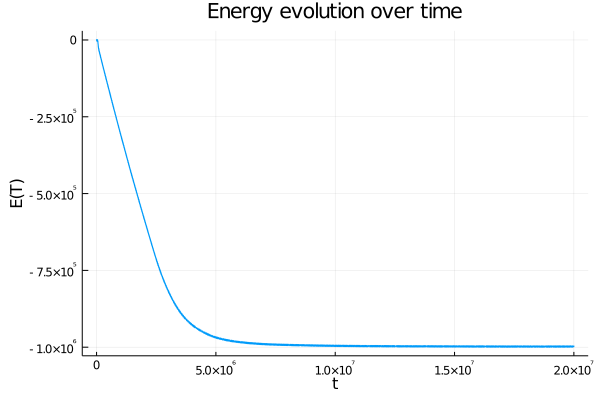
\includegraphics[width=0.65\linewidth]{figures/pop1000/energy_evolution_1-2_10e7.png}
\caption{\textit{{\small Total system energy evolution over time for a simulation of final model ran for $t=2\cdot 10^7$ over a population of 1000}}}
\label{pop1000:evol}
\end{figure}

Figure \ref{pop1000:evol} shows the evolution of the total system energy for this simulation. Energetically, the system reaches the ground state at $t\approx5\cdot 10^6$. However, consensus is reached much earlier ($t\approx10^5$), as figure \ref{pop1000:partition} reveals. This indicates that the network rewiring dynamics bring their own contribution to the total energy. The issue of different rewiring frequencies will be analysed in section 3.2. Refer to figure \ref{pop1000} for all the plots for this simulation.\\

\begin{figure}[!ht]
\centering
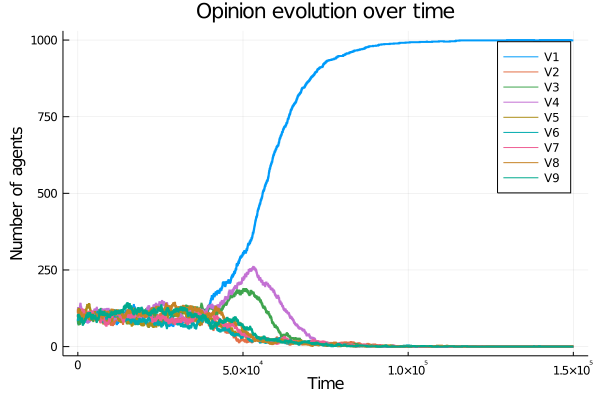
\includegraphics[width=0.65\linewidth]{figures/pop1000/opinion_evolution_1-15_10e4.png}
\caption{\textit{{\small Opinion partition over time, $t \in \{1..1.5\cdot 10^5\}$}}}
\label{pop1000:partition}
\end{figure}

\section{Fixed rewiring probability}

When the rewiring probability $\eta$ is fixed, consensus is reached more slowly, even if the population itself is smaller, as revealed by figure \ref{2_2:partition}, where consensus wasn't yet reached by the end of the simulation at $t=1.8\cdot 10^6$.\\

\begin{table}[!ht]
\centering
\begin{small}
\caption{\textit{Specifications for fixed rewiring probability simulation run}}
\begin{tabular}{ccc}
\hline
Initial network             & Barabási–Albert network\\
Opinion dynamics            & Potts model \\
Rewiring probability        & $\eta_{i,j}=0.5$\\
Run time                    & $t=1.8\cdot 10^6$\\
Temperature                 & $T=1$ \\
Coupling constant           & $J=1$ \\
Population                  & $N=100$\\
\hline
\label{fixed-rewiring-specs}
\end{tabular}
\end{small}
\end{table}




A possible explanation for the slower opinion dynamics is that the randomness of the rewiring caused by the fixed $\eta$ makes it harder for the agents to have the same neighbors for too long, thus adding more noise to the dynamics.\\

\begin{figure}[!ht]
\centering
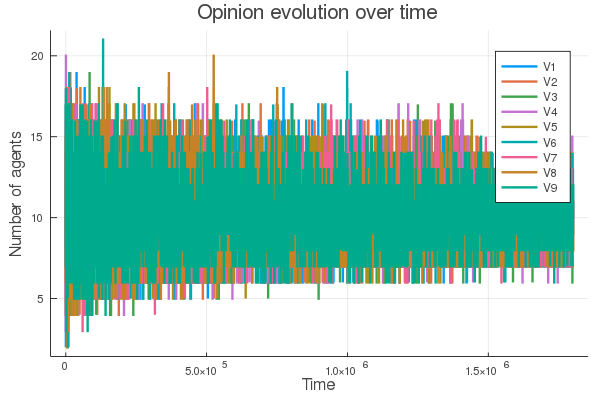
\includegraphics[width=0.65\linewidth]{figures/2_2/vote_evolution.png}
\caption{\textit{{\small Opinion partition over time for simulation ran for $t=1.8\cdot 10^6$ over a population of 100}}}
\label{2_2:partition}
\end{figure}

Refer to figure \ref{2_2} for all the plots for this simulation.

\subsection{Majority rule}

A variant of the fixed rewiring probability simulation is the majority rule simulation. In this scenario, the opinion dynamics step behaves as follows:\\

\begin{enumerate}
    \item An agent is selected at random.
    \item The opinions of its inneighbors are counted.
    \item The agent copies the opinion held by the majority of its inneighbors.
\end{enumerate}

\vspace{14pt}

\begin{table}[!ht]
\centering
\begin{small}
\caption{\textit{Specifications for majority rule run}}
\begin{tabular}{ccc}
\hline
Initial network             & Barabási–Albert network\\
Opinion dynamics            & Majority rule \\
Rewiring probability        & $\eta_{i,j}=0.5$\\
Run time                    & $t=10^6$\\
Temperature                 & $T=1$ \\
Coupling constant           & $J=1$ \\
Population                  & $N=100$\\
\hline
\label{majority-rule-specs}
\end{tabular}
\end{small}
\end{table}




Unsurprisingly, in this case consensus is reached almost immediately, despite the noise generated by network rewiring (see figure \ref{2_1:partition}). This opinion dynamics rule is even stronger than a Potts rule with $T=0$, since in that case there are still chances that the new opinion will cause an increase in system energy, and as such it is dropped.\\

\begin{figure}[!ht]
\centering
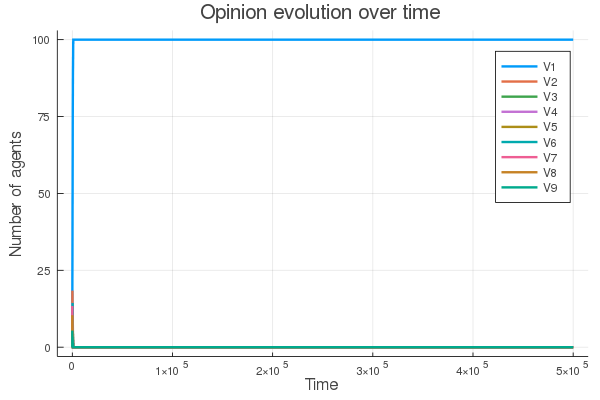
\includegraphics[width=0.65\linewidth]{figures/2_1/vote_evolution.png}
\caption{\textit{{\small Opinion partition over time for majority rule simulation ran for $t=10^6$ over a population of 100}}}
\label{2_1:partition}
\end{figure}

Refer to figure \ref{2_1} for all the plots for this simulation.

\subsection{Random initial network}

Another tested variant to the fixed rewiring probability simulation is one where the network is initialized using a 
Erdős–Rényi random network\cite{bollobas_bela_2004}.\\

\begin{table}[!ht]
\centering
\begin{small}
\caption{\textit{Specifications for Erdős–Rényi initial network run}}
\begin{tabular}{ccc}
\hline
Initial network             & Erdős–Rényi network\\
Opinion dynamics            & Potts model \\
Rewiring probability        & $\eta_{i,j}=0.5$\\
Run time                    & $t=2\cdot 10^6$\\
Temperature                 & $T=1$ \\
Coupling constant           & $J=1$ \\
Population                  & $N=100$\\
\hline
\label{er-specs}
\end{tabular}
\end{small}
\end{table}




In this case, the results (figure \ref{2_1_er:partition}) are rather similar to the results obtained from using a Barabási–Albert. This confirms that the network rewiring dynamics are strong enough so as to be independent of the topology of the initial network.\\

\begin{figure}[!htb]
\centering
\begin{subfigure}{0.49\linewidth}
    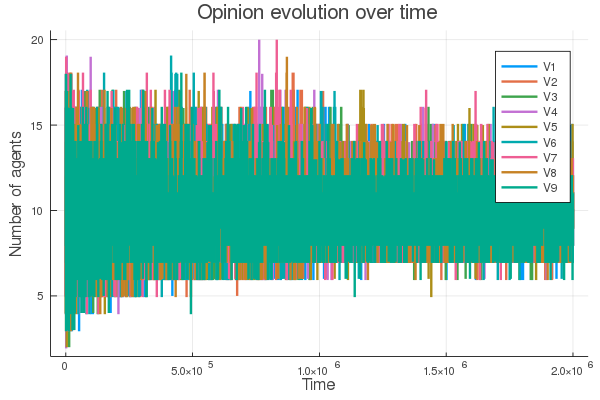
\includegraphics[width=\linewidth]{figures/2_2_er/vote_evolution.png}
    \caption{\textit{{\small Opinion partition over time}}}
    \label{2_1_er:partition}
\end{subfigure}
\begin{subfigure}{0.49\linewidth}
    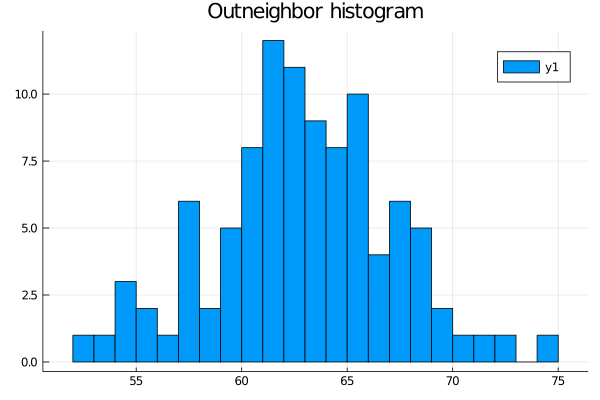
\includegraphics[width=\linewidth]{figures/2_2_er/OutneighborHistogram.png}
    \caption{\textit{{\small Outneighbor histogram}}}
    \label{2_1_er:histogram}
\end{subfigure}
\caption{\textit{{\small Opinion partition and outneighbor histogram for random initial network simulation ran for $t=2\cdot 10^6$ over a population of 100}}}
\end{figure}

Refer to figure \ref{2_2_er} for all the plots for this simulation.

\section{Varying rewiring frequency}

Keeping the same fixed rewiring probability $\eta=0.5$, four simulations were experimenting with different rewiring frequencies. Instead of running the rewiring procedure every step of the simulation, the procedure was run at every 10, 50, 100, and 1000 steps, respectively (see table \ref{rew-specs}).\\

\begin{table}[!ht]
\centering
\begin{small}
\caption{\textit{Specifications for different rewiring frequencies simulation runs}}
\begin{tabular}{ccc}
\hline
Initial network             & Barabási–Albert network\\
Opinion dynamics            & Potts model \\
Rewiring probability        & $\eta_{i,j}=0.5$\\
Run time                    & $t=1.4\cdot 10^5, 2\cdot 10^6, 4.2\cdot 10^6, 2\cdot 10^6, 6.5\cdot 10^6$\\
Temperature                 & $T=1$ \\
Coupling constant           & $J=1$ \\
Population                  & $N=100$\\
Rewiring frequency          & $1/10, 1/50, 1/100, 1/1000, 0$ \\
\hline
\label{rew-specs}
\end{tabular}
\end{small}
\end{table}




Analysing the results (figure \ref{2_2_rew:all}), it appears, however, that even with a fixed $\eta$, the network rewiring is involved in reaching the energy ground state. The lower the rewiring frequency is, the higher the noise and the higher the minimal system energy.\\

\begin{figure}[!htb]
\centering
\begin{subfigure}{0.47\linewidth}
    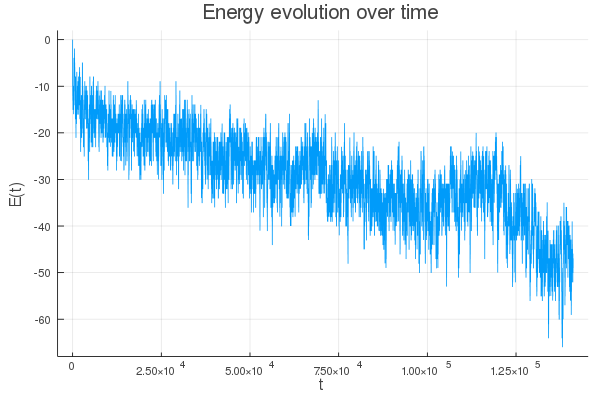
\includegraphics[width=\linewidth]{figures/2_2_10rew/energy_evolution.png}
    \caption{Rewiring every 10 steps}
\end{subfigure}
\begin{subfigure}{0.47\linewidth}
    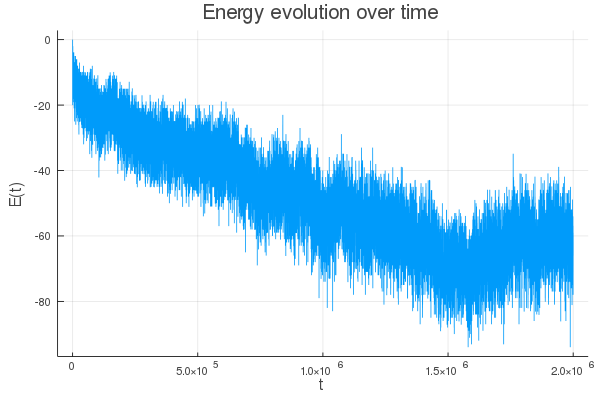
\includegraphics[width=\linewidth]{figures/2_2_50rew/energy_evolution.png}
    \caption{Rewiring every 50 steps}
\end{subfigure}
\begin{subfigure}{0.47\linewidth}
    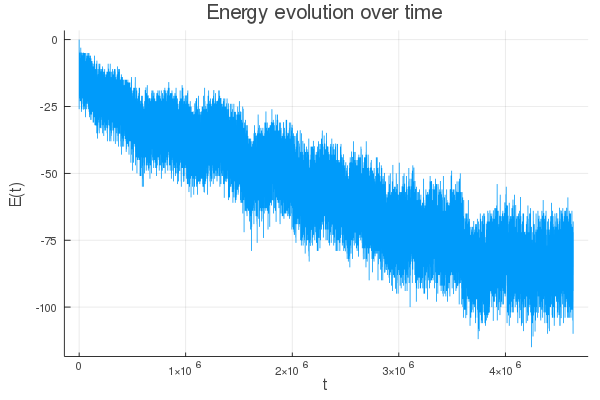
\includegraphics[width=\linewidth]{figures/2_2_100rew/energy_evolution.png}
    \caption{Rewiring every 100 steps}
\end{subfigure}
\begin{subfigure}{0.47\linewidth}
    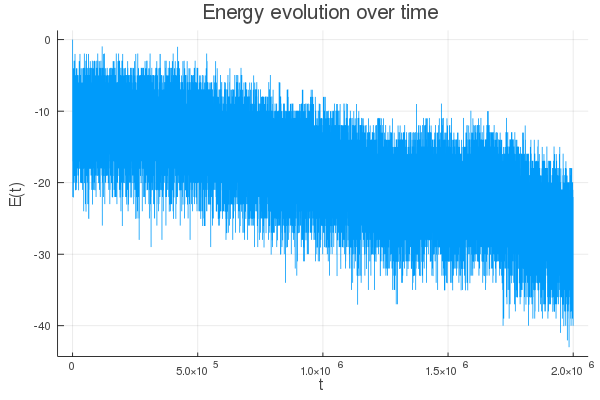
\includegraphics[width=\linewidth]{figures/2_2_1000rew/energy_evolution.png}
    \caption{Rewiring every 1000 steps}
\end{subfigure}
\begin{subfigure}{0.47\linewidth}
    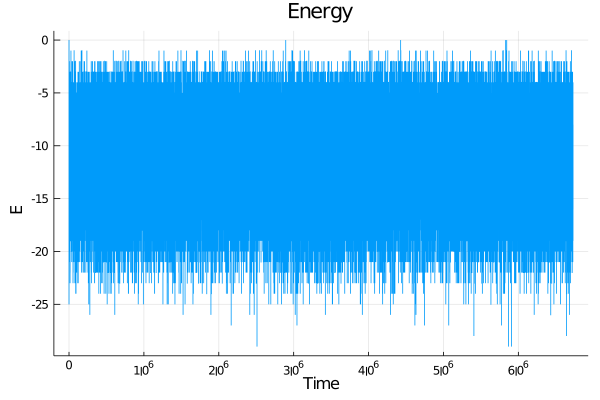
\includegraphics[width=\linewidth]{figures/no_rew/Energy_norewire2.png}
    \caption{No rewiring}
\end{subfigure}
\caption{\textit{{\small Simulations ran for different rewiring frequencies over a population of 100}}}
\label{2_2_rew:all}
\end{figure}

\section{Varying temperature}

Similar to the previous the section, simulations were also done with varying temperatures $T$. Again, $\eta$ was fixed and the population was 100 (see table \ref{T-specs}).\\

Figure \ref{2_2_t1:ener_inne} shows the energy evolution and the opinion partition over time for a system at $T=1$. Figures \ref{2_2_t10:ener_inne} and \ref{2_2_t100:ener_inne} show the same information for simulations ran at $T=10$, and $T=100$, respectively. Additional plots, such as energy distribution plots, can be found in the appendix figures \ref{2_2_t1}, \ref{2_2_t10}, and \ref{2_2_t100}.\\

\begin{table}[!ht]
\centering
\begin{small}
\caption{\textit{Specifications for different temperatures simulation runs}}
\begin{tabular}{ccc}
\hline
Initial network             & Barabási–Albert network\\
Opinion dynamics            & Potts model \\
Rewiring probability        & $\eta_{i,j}=0.5$\\
Run time                    & $t=6\cdot 10^6$\\
Temperature                 & $T=1,10,100$ \\
Coupling constant           & $J=1$ \\
Population                  & $N=100$ \\
\hline
\label{T-specs}
\end{tabular}
\end{small}
\end{table}

Here, three trends are apparent. First, higher temperature is correlated with higher noise. This should come as no surprise, especially when considering the expression of opinion switch probability $p$ (\ref{switch_prob}). Indeed, this mirrors the classic Ising behaviour presented in section 1.1. It is still an important confirmation of the fact temperature behaves as expected in this model, and thus can be easily related to tolerance.\\

\begin{figure}[!htb]
\centering
\begin{subfigure}{0.47\linewidth}
    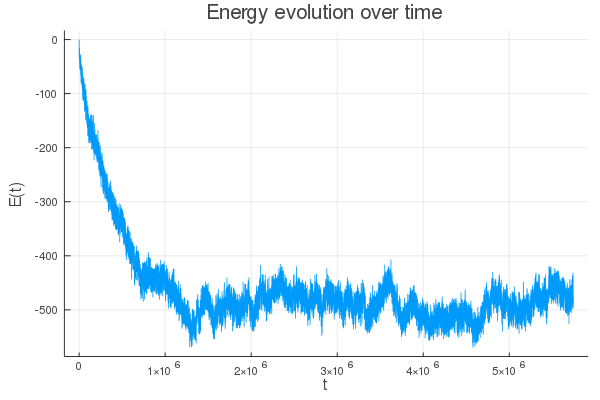
\includegraphics[width=\linewidth]{figures/2_2_t1/energy_evolution.png}
    \caption{Total system energy evolution over time}
\end{subfigure}
\begin{subfigure}{0.47\linewidth}
    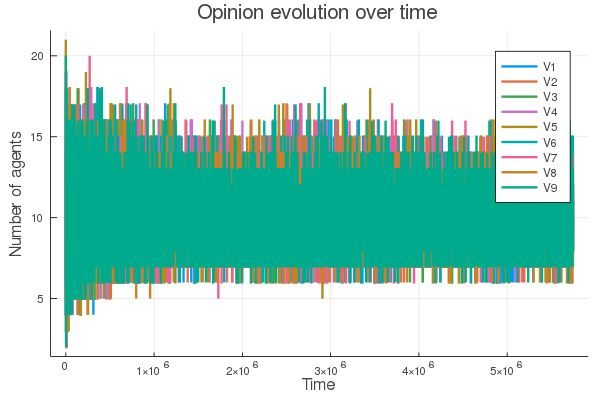
\includegraphics[width=\linewidth]{figures/2_2_t1/vote_evolution.png}
    \caption{Opinion partition over time}
\end{subfigure}
\caption{\textit{{\small Simulation with fixed rewiring probability, ran for $t=6\cdot 10^6$ at $T=1$, over a population of 100}}}
\label{2_2_t1:ener_inne}
\end{figure}

Secondly, the evolution of opinions over time exhibits a chaotic behaviour for $T=10$ and $T=100$, while for $T=1$ it seems like it may be convergent, though a longer run would have been necessary to confirm this beyond all doubts. However, it can still be observed that for $T=1$ the share of opinions in the network is more evenly divided, hence the smaller values in the opinion partition plot (figure \ref{2_2_t1:ener_inne}).\\

\begin{figure}[!htb]
\centering
\begin{subfigure}{0.47\linewidth}
    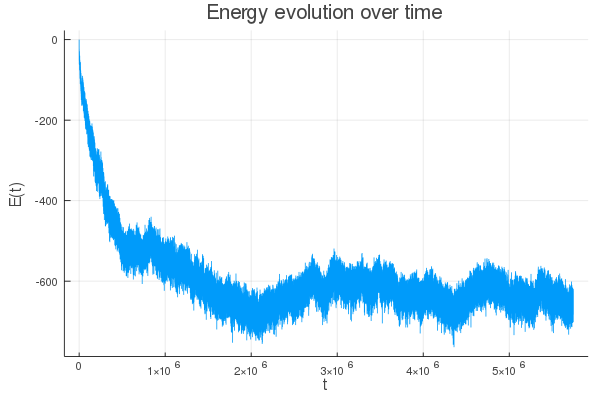
\includegraphics[width=\linewidth]{figures/2_2_t10/energy_evolution.png}
    \caption{Total system energy evolution over time}
\end{subfigure}
\begin{subfigure}{0.47\linewidth}
    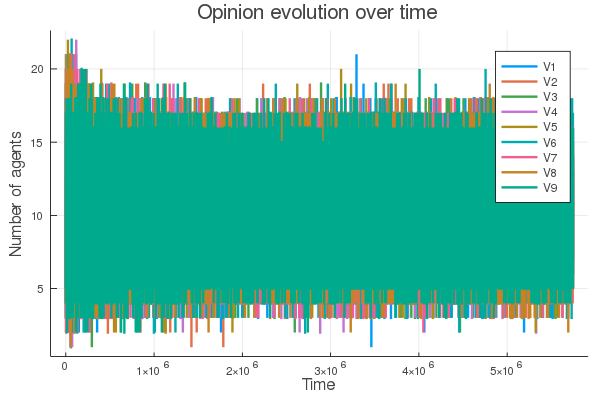
\includegraphics[width=\linewidth]{figures/2_2_t10/vote_evolution.png}
    \caption{Opinion partition over time}
\end{subfigure}
\caption{\textit{{\small Simulation with fixed rewiring probability, ran for $t=6\cdot 10^6$ at $T=10$, over a population of 100}}}
\label{2_2_t10:ener_inne}
\end{figure}


Thirdly, and most interestingly, the higher the temperature, the lower the system energy ground state seems to be. If for $T=1$ it is $\langle E_{ground} \rangle\approx490$, for $T=10$, it is $\langle E_{ground} \rangle\approx610$, and for $T=100$, it is $\langle E_{ground} \rangle\approx650$. This has interesting implications, as higher tolerance could mean, in this context, a more stable configuration of the social network.\\

\begin{figure}[!htb]
\centering
\begin{subfigure}{0.47\linewidth}
    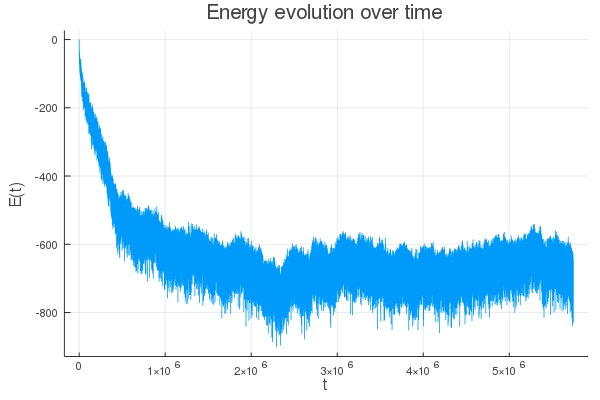
\includegraphics[width=\linewidth]{figures/2_2_t100/energy_evolution.png}
    \caption{Total system energy evolution over time}
\end{subfigure}
\begin{subfigure}{0.47\linewidth}
    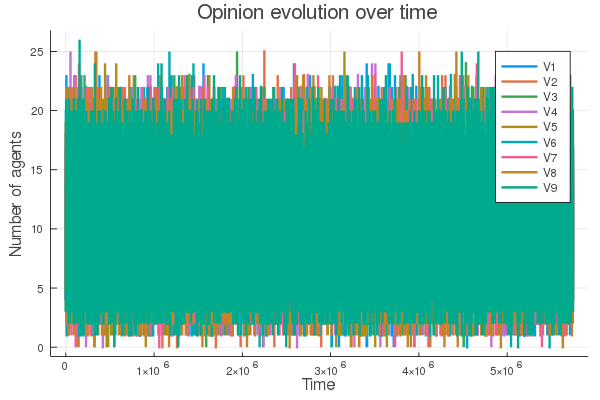
\includegraphics[width=\linewidth]{figures/2_2_t100/vote_evolution.png}
    \caption{Opinion partition over time}
\end{subfigure}
\caption{\textit{{\small Simulation with fixed rewiring probability, ran for $t=6\cdot 10^6$ at $T=100$, over a population of 100}}}
\label{2_2_t100:ener_inne}
\end{figure}

\chapter{Conclusions}

The most important contribution of this thesis is to provide an alternative and --- in my opinion --- more realistic approach to model opinion dynamics compared to single-layered models. The new approach is based on the postulate that people are influenced by others with already compatible views. The process of selecting the persons one is willing to listen to can ultimately be the factor that leads to consensus, polarization, or otherwise fragmentation. In the two-layered model, agents change their opinions in order to be more in line with their neighbors, while at the same time the network is constantly changing in order to link agents with similar values.\\

I show that the outcome depends strongly on the fashion and frequency to which the network is updated. A random rewiring dynamic will cause high noise and prolonged fragmentation, while a dynamic based on similarity between agents ultimately leads to consensus. A lower network update ratio will lead to a slower evolution towards system stability and to higher noise in the evolution of opinions. Furthermore, temperature variations evoke the expected behaviour from an Ising-like simulation.\\

Admittedly, the model is still a long way from maturity, with the analytical descriptions of its behaviour still needing to be done. The exact relationship between the time required to reach the system energy ground state and rewiring frequency is sill unknown, as is the value of critical temperature $T_C$ under default conditions. Besides a better description of the model phenomenology, future steps can include experimenting with different cultural values distributions. While it might be interesting to study models in themselves, ultimately they have to work for the reasons they were created, in this regard it would be a good idea to test the model on networks extracted from empirical data.\\







\renewcommand{\contentsname}{References}
\renewcommand\bibname{References} %
\addcontentsline{toc}{chapter}{References}
\markboth{References}{References} %
\bibliographystyle{unsrt}
%
%\bibliographystyle{plain}

\bibliography{References}

\begin{appendices}
\chapter{Simulation Code}

\section{SocialSim.jl}
\begin{lstlisting}[language=julia]
module SocialSim

using Dates
using Random
using LightGraphs
using DataFrames
using CSV
using Dates
using GraphIO
using Plots
using StatsBase
using ProgressMeter

export run_sim

const J = 1

include("init.jl")
include("analysis.jl")
include("dynamics.jl")
include("storage.jl")

#Runs the simulation at a determined temperature for a determined number of steps
function run_sim(T,population,steps; exports_number=10)
    
    #Random.seed!(1234)

    #Get time of simulation and prepare folders
    exportTime = Dates.format(Dates.now(), "yyyy-mm-ddTHH-MM-SS")
    mkdir("Data/$exportTime")
    mkdir("Data/$exportTime/Network")

    
    #Initializing network and data frame
    data = createDataFrame()
    network, nodes = initNetwork(data, population)

    #Export network at each nx steps
    nx = div(steps, exports_number) 

    #Executing steps
    @showprogress 5 "Computing..." for i in 1:steps
        ni = rand(1:population)
        procedure2(nodes, network, data, ID=ni, N=population, T=T)

        if mod(i, nx) == 0
            exportNetwork(exportTime, network, nodes, i)
        end
    end

    #Export data to a new folder
    exportData(exportTime, data, network, nodes)
    plotAnalysis(steps, exportTime, data, nodes, network)
end

#Runs the simulation at T for a determined time interval (in hours)
#=function set_run(T,population,duration; exports_number=10)
    
    #Get time of simulation and prepare folders
    exportTime = Dates.format(Dates.now(), "yyyy-mm-ddTHH-MM-SS")
    mkdir("Data/$exportTime")
    mkdir("Data/$exportTime/Network")
    
    #Initializing network and data frame
    data = createDataFrame()
    network, nodes = initNetwork(data, population)

    #Export network at each nx steps
    nx = div(steps, exports_number) 

    timelimit = Dates.now() + Dates.Minute(duration)
    
    #Executing steps
    while Dates.now() < timelimit #&& length(Data.E) <= 2000000
        ni = rand(1:population)
        procedure2(nodes, network, data, ID=ni, N=population, T=T)

        if mod(i, nx) == 0
            exportNetwork(exportTime, network, nodes, i)
        end
    end

    #Export data to a new folder
    exportData(exportTime)
    plotAnalysis(length(data.E)-1, exportTime)
end=#

end

\end{lstlisting}

\vspace{14pt}

\section{init.jl}
\begin{lstlisting}[language=julia]
struct Agent{T,E}
    id::Int
    values::Vector{T}
    vote::Ref{Int}
    energy::Ref{E}
end

function initNetwork(data, N)
    #Generate Barabasi graph with N nodes, 3 conntections each, 10 initial nodes
    network = barabasi_albert(N, 10, 3, #=seed=1,=# is_directed=true)
    #global Network = erdos_renyi(N, 4, is_directed=true)
    
    #Initialize agents
    nodes = Agent{Int,Int}[]
    for i in 1:N
        push!(nodes, Agent(i, rand(0:10, 5), Ref(rand(1:10)), Ref(0)))
    end
    
    #Initialize energy
    for i in 1:N
        dE!(nodes, i, network)
    end
    computeEnergy!(data, nodes)

    #Count initial preferences
    trackPreference!(data, nodes)

    return network, nodes
end

\end{lstlisting}

\vspace{14pt}

\section{dynamics.jl}
\begin{lstlisting}[language=julia]
function rewire!(network, nodes, ID, options; remove=false)
    isempty(options) && return

    target = rand(options)
        
    # number of values
    val_range = axes(nodes[ID].values, 1)
    val_norm = 1 / (val_range[end] * 10)
    p = val_norm * sum(
        i->abs(nodes[ID].values[i]-nodes[target].values[i]),
        val_range)
    if !remove
        p = 1 - p
    end

    if rand() <= p
        #Add pr remove edge
        if remove
            rem_edge!(network, target, ID)
        else
            add_edge!(network, target, ID)
        end

        #Adjust energy
        if nodes[target].vote[] == nodes[ID].vote[]
            j = remove ? J : -J
            nodes[ID].energy[] += j
        end
    end
end

function procedure2(nodes, network, data; ID, N, T)   

    #Add new row to data frame
    push!(data, zeros(10+1))

    #Select unconnected node, connect with probability w
    options = Int[]
    for i in 1:N
        if has_edge(network, i, ID) == false
            push!(options, i)
        end
    end

    rewire!(network, nodes, ID, options, remove=false)
    
    #Select edge, disconnect with probabilty w^-1
    options = inneighbors(network, ID)

    rewire!(network, nodes, ID, options, remove=true)

    #Select new random preference & track preference change
    oldVal = nodes[ID].vote[]
    newVal = rand(1:10)
    nodes[ID].vote[] = newVal

    #Substract current node energy from former node energy
    deltaE = dE(nodes, ID, network) - nodes[ID].energy[]
    
    p = -(deltaE)/T

    #If deltaE<0 apply it:
    if deltaE < 0
        nodes[ID].energy[] += deltaE    
        for i in outneighbors(network, ID)
            nodes[i].energy[] = dE(nodes, i, oldVal, newVal)
        end
    #If deltaE>0 apply it with following probability:
    elseif rand() < exp(p)
        nodes[ID].energy[] += deltaE
        for i in outneighbors(network, ID)
            nodes[i].energy[] = dE(nodes, i, oldVal, newVal)
        end
    else
        nodes[ID].vote[] = oldVal
    end

    #Log preferences
    trackPreference!(data, oldVal, nodes[ID].vote[])

    #Compute system energy
    computeEnergy!(data, nodes)


    #Optional: change core opinions
end

\end{lstlisting}

\vspace{14pt}

\section{analysis.jl}
\begin{lstlisting}[language=julia]
"""
    computeEnergy!(data, nodes)

Compute sytem energy
"""
function computeEnergy!(data, nodes)
    E = 0
    for i in 1:length(nodes)
        data.E[end] += nodes[i].energy[]
    end
end

"""
    dE(ID,oldVal,newVal)

Computes node energy by assessing the change in preference of an inneighbor
"""
function dE(nodes, ID, oldVal, newVal)

    if newVal == nodes[ID].vote[] && oldVal == nodes[ID].vote[]
        epsilon = nodes[ID].energy[]
    elseif newVal == nodes[ID].vote[] && oldVal != nodes[ID].vote[]
        epsilon = nodes[ID].energy[] - J
    elseif newVal != nodes[ID].vote[] && oldVal == nodes[ID].vote[]
        epsilon = nodes[ID].energy[] + J
    else
        epsilon = nodes[ID].energy[]
    end

    return epsilon
end

function dE(nodes, ID, network)

    #Goes through inneighbors and computes Potts node energy (epsilon)
    options = inneighbors(network,ID)
    epsilon = 0
    for i in 1:length(options)
        if nodes[ID].vote[] == nodes[options[i]].vote[]
            epsilon += -J
        end
    end

    return epsilon
end

#Slower: recomputes node energy thoroughly
function dE!(nodes, ID, network)

    epsilon = dE(nodes, ID, network)
    #Assign node energy
    nodes[ID].energy[] = epsilon
end

function datacol(data, i)
    getproperty(data, Symbol("c$i"))
end

"""
    trackPreference!(data, nodes)

Count popularity of each candidate
"""
function trackPreference!(data, nodes)
    for i in 1:length(nodes)
        v = nodes[i].vote[]
        
        # data.c$v[end] += 1
        datacol(data, v)[end] += 1
    end
end

function trackPreference!(data, old, new)
    #Copy previous distribution
    for i=1:10
        datacol(data, i)[end] = datacol(data, i)[end-1]
    end

    #Remove old value
    datacol(data, old)[end] -= 1
    #Add new value
    datacol(data, new)[end] += 1
end

#Plotting
function plotAnalysis(t, dir, data, nodes, network)

    #Energy evolution
    plot1=plot(1:t+1, data.E[1:t+1]#=/Data.E[1]=#, legend=false)
    xlabel!("Time")
    ylabel!("E/E_0")
    title!("Energy")
    png("Data/$dir/Energy")

    #Energy distribution
    energyDistribution=counts(-data.E)
    plot2=plot(1:length(energyDistribution), energyDistribution, legend=false)
    title!("Energy distribution")
    png("Data/$dir/EnergyDistribution")

    #Inneighbor histogram
    noInneighbors = []
    for i in 1:length(nodes)
        push!(noInneighbors, length(inneighbors(network, i)))
    end
    plot3=histogram(noInneighbors, bins = 15)
    title!("Inneighbor histogram")
    png("Data/$dir/InneighborHistogram")
end

\end{lstlisting}

\vspace{14pt}

\section{storage.jl}
\begin{lstlisting}[language=julia]
function createDataFrame()
    DataFrame(E=[0], c1=[0], c2=[0], c3=[0], c4=[0], c5=[0], c6=[0], c7=[0], c8=[0], c9=[0], c10=[0])
end

function exportData(dir, data, network, nodes) 
    #Save log
    CSV.write("Data/$dir/data.csv", data)

    #Save nodes table
    nodes_df = DataFrame(ID = Int[], Vote = Int[], sigma_1 = Int[], sigma_2 = Int[], sigma_3 = Int[], 
        sigma_4 = Int[], sigma_5 = Int[], E = Int[])
    
    for i in 1:length(nodes)
        push!(nodes_df, (nodes[i].id, nodes[i].vote[], nodes[i].values[1], nodes[i].values[2], 
            nodes[i].values[3], nodes[i].values[4], nodes[i].values[5], nodes[i].energy[]))
    end

    CSV.write("Data/$dir/nodes.csv", nodes_df)

    #Exporting the graph
    savegraph("Data/$dir/graph.net", network, "Network", GraphIO.NET.NETFormat())
end

function exportNetwork(dir, network, nodes, step)
    #Save nodes table
    nodes_df = DataFrame(ID = Int[], Vote = Int[], sigma_1 = Int[], sigma_2 = Int[], sigma_3 = Int[], 
        sigma_4 = Int[], sigma_5 = Int[], E = Int[])
    
    for i in 1:length(nodes)
        push!(nodes_df, (nodes[i].id, nodes[i].vote[], nodes[i].values[1], nodes[i].values[2], 
            nodes[i].values[3], nodes[i].values[4], nodes[i].values[5], nodes[i].energy[]))
    end

    CSV.write("Data/$dir/Network/nodes_$step.csv", nodes_df)

    #Exporting the graph
    savegraph("Data/$dir/Network/graph_$step.net", network, "Network", GraphIO.NET.NETFormat())
end

\end{lstlisting}

\vspace{14pt}

\chapter{Plots}

\begin{figure}[!htb]
\centering
\begin{subfigure}{0.47\linewidth}
    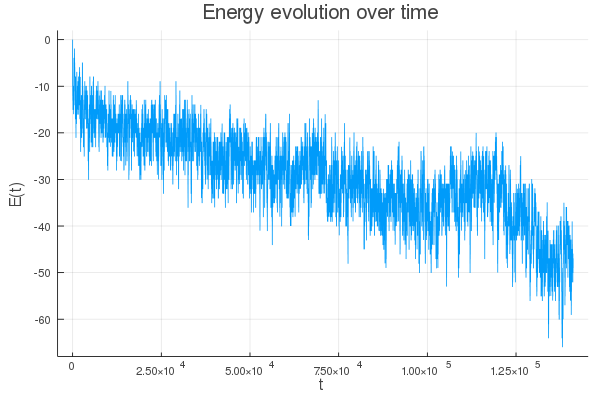
\includegraphics[width=\linewidth]{figures/2_2_10rew/energy_evolution.png}
    \caption{Rewiring every 10 steps}
\end{subfigure}
\begin{subfigure}{0.47\linewidth}
    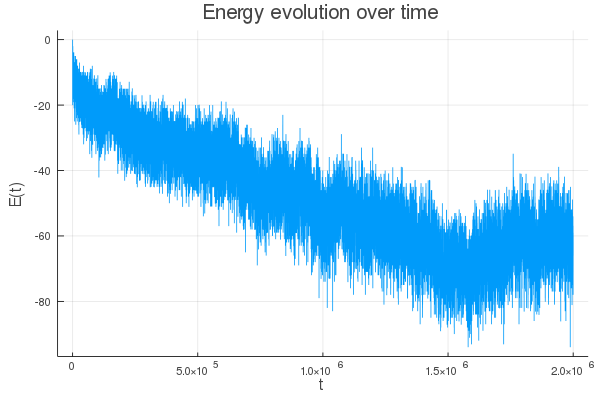
\includegraphics[width=\linewidth]{figures/2_2_50rew/energy_evolution.png}
    \caption{Rewiring every 50 steps}
\end{subfigure}
\begin{subfigure}{0.47\linewidth}
    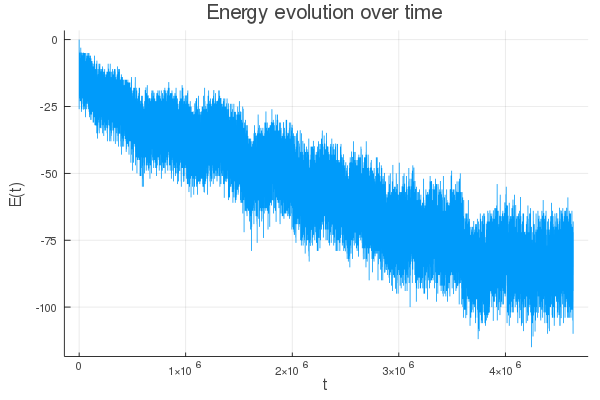
\includegraphics[width=\linewidth]{figures/2_2_100rew/energy_evolution.png}
    \caption{Rewiring every 100 steps}
\end{subfigure}
\begin{subfigure}{0.47\linewidth}
    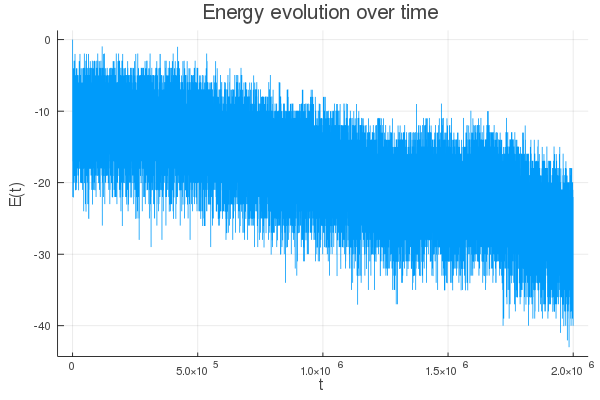
\includegraphics[width=\linewidth]{figures/2_2_1000rew/energy_evolution.png}
    \caption{Rewiring every 1000 steps}
\end{subfigure}
\begin{subfigure}{0.47\linewidth}
    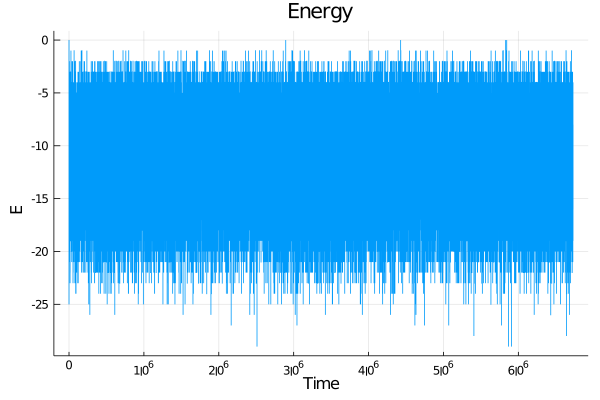
\includegraphics[width=\linewidth]{figures/no_rew/Energy_norewire2.png}
    \caption{No rewiring}
\end{subfigure}
\caption{\textit{{\small Simulations ran for different rewiring frequencies over a population of 100}}}
\label{2_2_rew}
\end{figure}

\begin{figure}
\centering
\begin{subfigure}[b]{0.65\linewidth}
    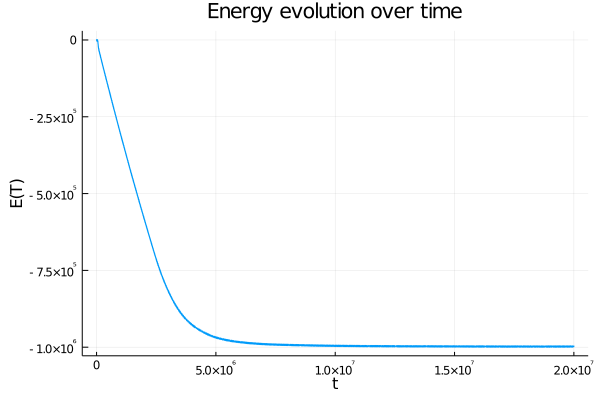
\includegraphics[width=\linewidth]{figures/pop1000/energy_evolution_1-2_10e7.png}
    \caption{Total system energy evolution over time}
\end{subfigure}
\begin{subfigure}[b]{0.65\linewidth}
    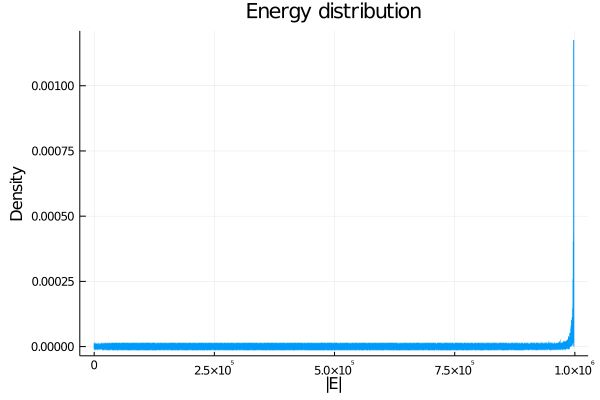
\includegraphics[width=\linewidth]{figures/pop1000/energy_distribution.png}
    \caption{Distribution of the absolute values of energy}
\end{subfigure}
\begin{subfigure}[b]{0.65\linewidth}
    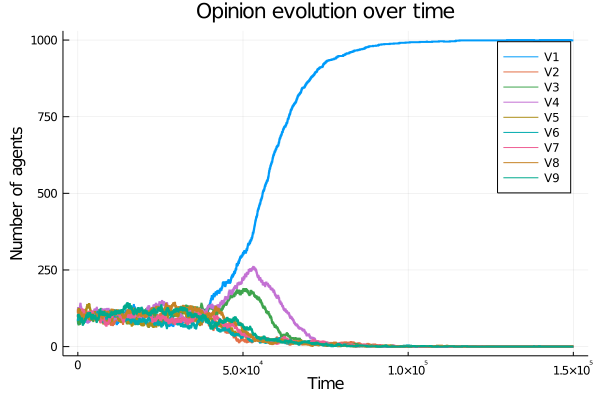
\includegraphics[width=\linewidth]{figures/pop1000/opinion_evolution_1-15_10e4.png}
    \caption{Opinion partition over time, $t \in \{1..1.5\cdot 10^5\}$}
\end{subfigure}
\caption{\textit{{\small Simulation of final model ran for $t=2\cdot 10^7$ over a population of 1000}}}
\label{pop1000}
\end{figure}

\begin{figure}[!htb]
\centering
\begin{subfigure}[b]{0.65\linewidth}
    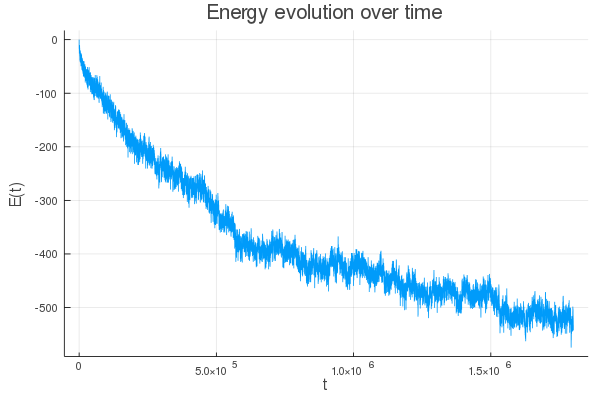
\includegraphics[width=\linewidth]{figures/2_2/energy_evolution.png}
    \caption{Total system energy evolution over time}
\end{subfigure}
\begin{subfigure}[b]{0.65\linewidth}
    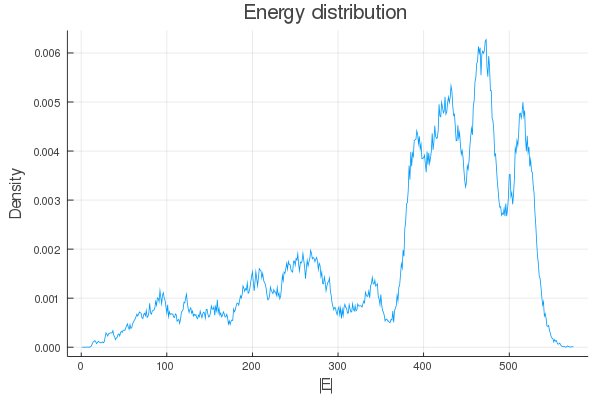
\includegraphics[width=\linewidth]{figures/2_2/energy_distribution.png}
    \caption{Distribution of the absolute values of energy}
\end{subfigure}
\begin{subfigure}[b]{0.65\linewidth}
    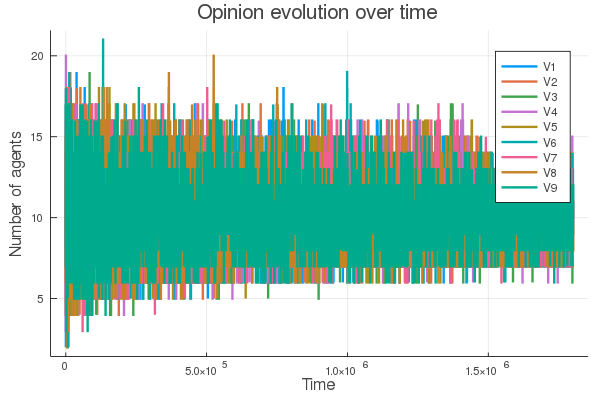
\includegraphics[width=\linewidth]{figures/2_2/vote_evolution.png}
    \caption{Opinion partition over time}
\end{subfigure}
\caption{\textit{{\small Fixed rewiring probability simulation ran for $t=1.8\cdot 10^6$ over a population of 100}}}
\label{2_2}
\end{figure}

\begin{figure}[!htb]
\centering
\begin{subfigure}[b]{0.65\linewidth}
    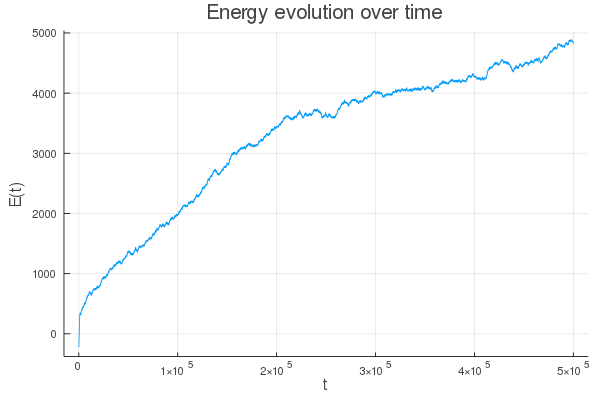
\includegraphics[width=\linewidth]{figures/2_1/energy_evolution.png}
    \caption{Total system energy evolution over time}
\end{subfigure}
\begin{subfigure}[b]{0.65\linewidth}
    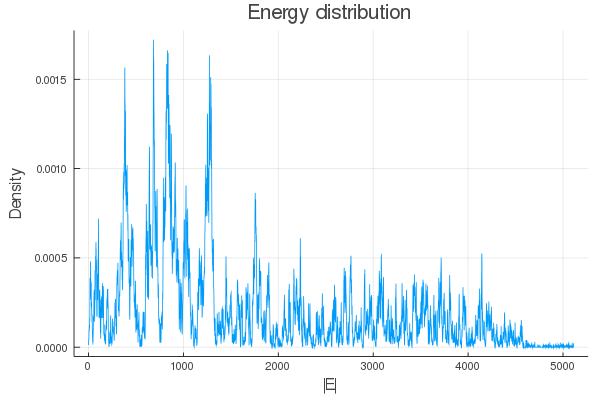
\includegraphics[width=\linewidth]{figures/2_1/energy_distribution.png}
    \caption{Distribution of the absolute values of energy}
\end{subfigure}
\begin{subfigure}[b]{0.65\linewidth}
    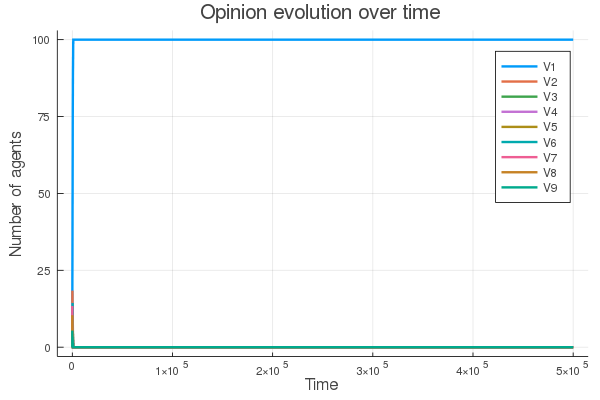
\includegraphics[width=\linewidth]{figures/2_1/vote_evolution.png}
    \caption{Opinion partition over time}
\end{subfigure}
\caption{\textit{{\small Majority rule simulation ran for $t=10^6$ over a population of 100}}}
\label{2_1}
\end{figure}

\begin{figure}[!htb]
\centering
\begin{subfigure}[b]{0.49\linewidth}
    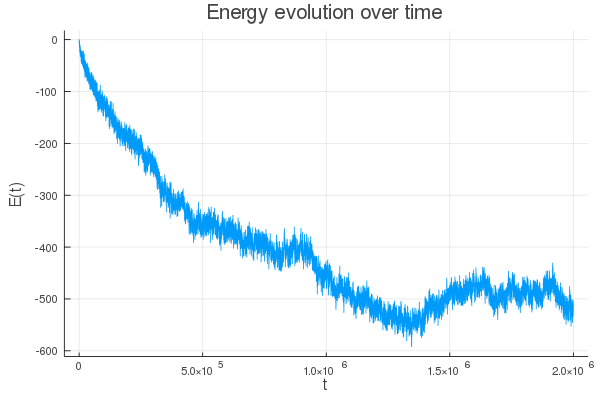
\includegraphics[width=\linewidth]{figures/2_2_er/energy_evolution.png}
    \caption{Total system energy evolution over time}
\end{subfigure}
\begin{subfigure}[b]{0.49\linewidth}
    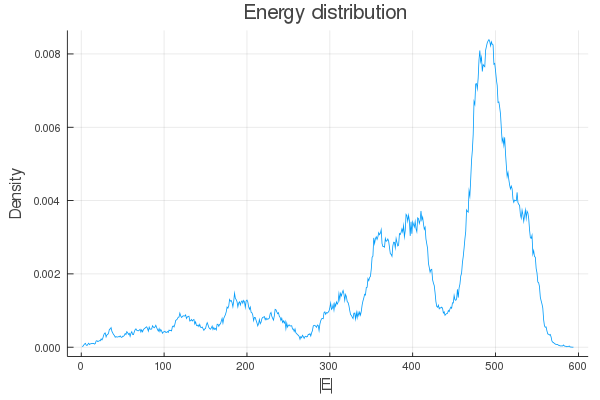
\includegraphics[width=\linewidth]{figures/2_2_er/energy_distribution.png}
    \caption{Distribution of the absolute values of energy}
\end{subfigure}
\begin{subfigure}[b]{0.49\linewidth}
    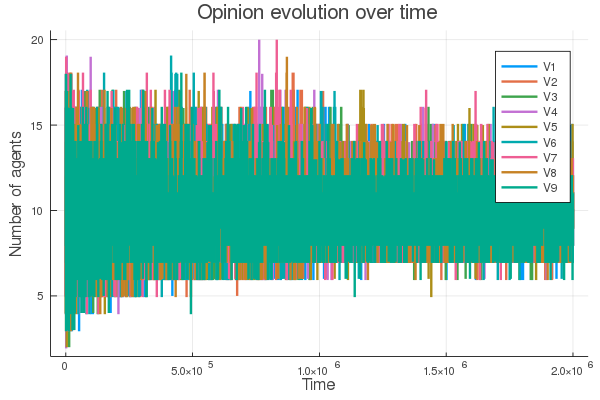
\includegraphics[width=\linewidth]{figures/2_2_er/vote_evolution.png}
    \caption{Opinion partition over time}
\end{subfigure}
\begin{subfigure}[b]{0.49\linewidth}
    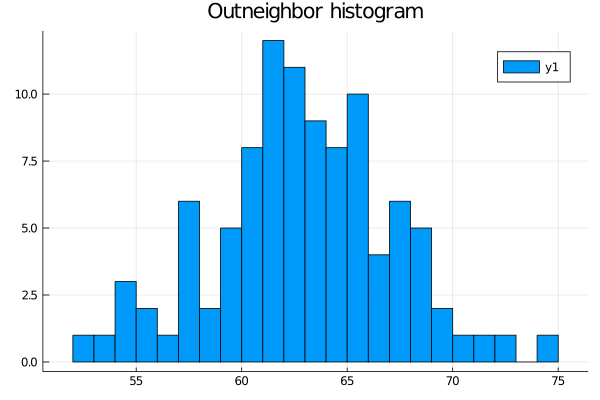
\includegraphics[width=\linewidth]{figures/2_2_er/OutneighborHistogram.png}
    \caption{Outneighbor histogram}
\end{subfigure}
\caption{\textit{{\small Random initial network simulation ran for $t=2\cdot 10^6$ over a population of 100}}}
\label{2_2_er}
\end{figure}

\begin{figure}[!htb]
\centering
\begin{subfigure}{0.47\linewidth}
    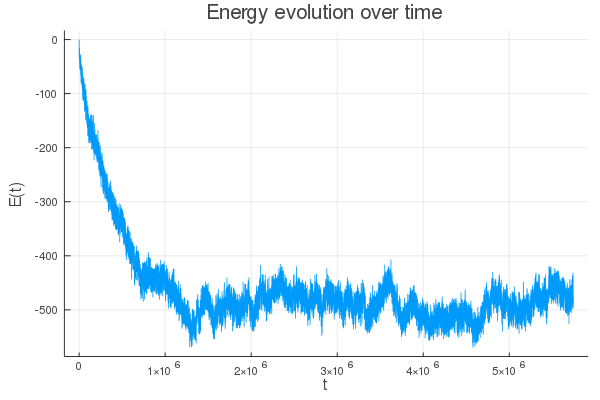
\includegraphics[width=\linewidth]{figures/2_2_t1/energy_evolution.png}
    \caption{Total system energy evolution over time}
\end{subfigure}
\begin{subfigure}{0.47\linewidth}
    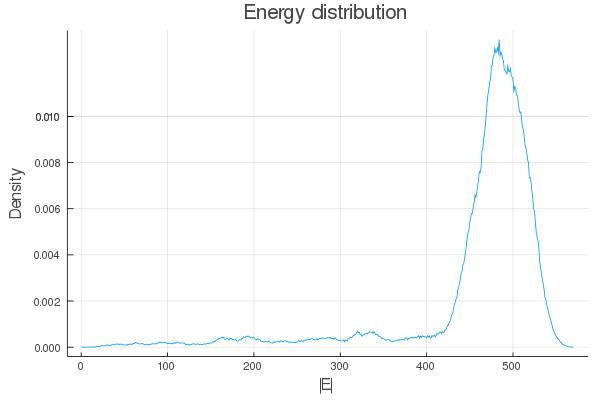
\includegraphics[width=\linewidth]{figures/2_2_t1/energy_distribution.png}
    \caption{Distribution of the absolute values of energy}
\end{subfigure}
\begin{subfigure}{0.47\linewidth}
    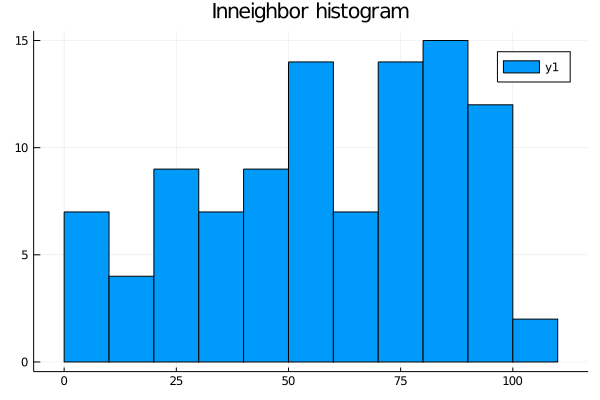
\includegraphics[width=\linewidth]{figures/2_2_t1/InneighborHistogram_temp=1.png}
    \caption{Inneighbor histogram}
\end{subfigure}
\begin{subfigure}{0.47\linewidth}
    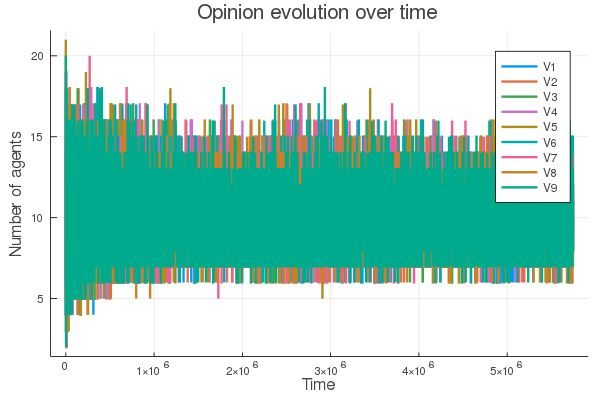
\includegraphics[width=\linewidth]{figures/2_2_t1/vote_evolution.png}
    \caption{Opinion partition over time}
\end{subfigure}
\caption{\textit{{\small Simulation with fixed rewiring probability, ran for $t=6\cdot 10^6$ at $T=1$, over a population of 100}}}
\label{2_2_t1}
\end{figure}

\begin{figure}[!htb]
\centering
\begin{subfigure}{0.47\linewidth}
    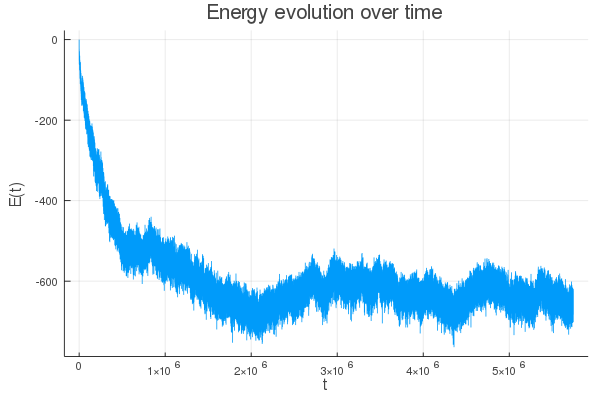
\includegraphics[width=\linewidth]{figures/2_2_t10/energy_evolution.png}
    \caption{Total system energy evolution over time}
\end{subfigure}
\begin{subfigure}{0.47\linewidth}
    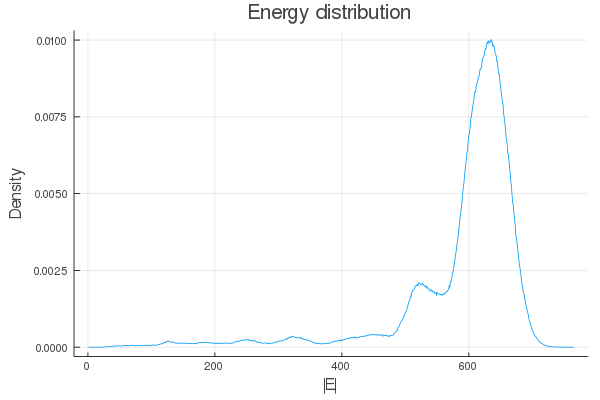
\includegraphics[width=\linewidth]{figures/2_2_t10/energy_distribution.png}
    \caption{Distribution of the absolute values of energy}
\end{subfigure}
\begin{subfigure}{0.47\linewidth}
    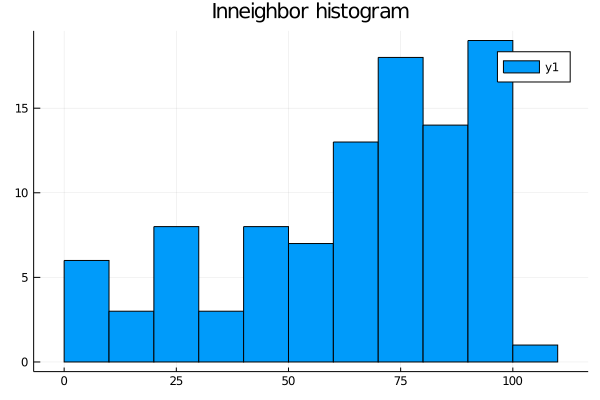
\includegraphics[width=\linewidth]{figures/2_2_t10/InneighborHistogram_temp=10.png}
    \caption{Inneighbor histogram}
\end{subfigure}
\begin{subfigure}{0.47\linewidth}
    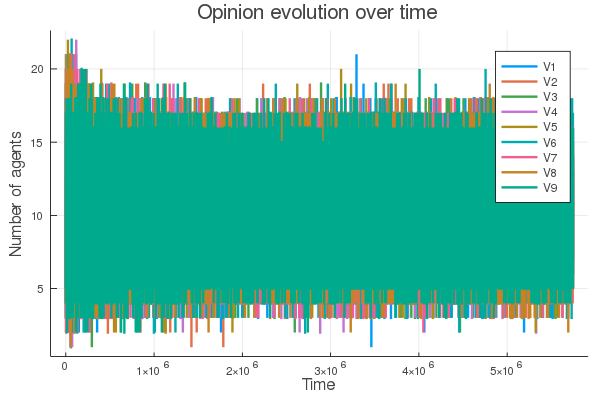
\includegraphics[width=\linewidth]{figures/2_2_t10/vote_evolution.png}
    \caption{Opinion partition over time}
\end{subfigure}
\caption{\textit{{\small Simulation with fixed rewiring probability, ran for $t=6\cdot 10^6$ at $T=10$, over a population of 100}}}
\label{2_2_t10}
\end{figure}

\begin{figure}[!htb]
\centering
\begin{subfigure}{0.47\linewidth}
    \includegraphics[width=\linewidth]{figures/2_2_t100/energy_evolution.png}
    \caption{Total system energy evolution over time}
\end{subfigure}
\begin{subfigure}{0.47\linewidth}
    \includegraphics[width=\linewidth]{figures/2_2_t100/energy_distribution.png}
    \caption{Distribution of the absolute values of energy}
\end{subfigure}
\begin{subfigure}{0.47\linewidth}
    \includegraphics[width=\linewidth]{figures/2_2_t100/InneighborHistogram_temp=100.png}
    \caption{Inneighbor histogram}
\end{subfigure}
\begin{subfigure}{0.47\linewidth}
    \includegraphics[width=\linewidth]{figures/2_2_t100/vote_evolution.png}
    \caption{Opinion partition over time}
\end{subfigure}
\caption{\textit{{\small Simulation with fixed rewiring probability, ran for $t=6\cdot 10^6$ at $T=100$, over a population of 100}}}
\label{2_2_t100}
\end{figure}

\end{appendices}

\end{document}
